\documentclass[a4paper, 12pt,openany]{book}  % aus KOMA-Skript, speziell für deutsche Texte interessant

\usepackage[ngerman]{babel}              % für die deutsche Sprache nach neuer Rechtschreibung

\usepackage[utf8]{inputenc}         % für die Nutzung deutscher Umlauten (Linux)
\linespread {1.10}\selectfont %1.25
%\usepackage[T1]{fontenc}  
\usepackage{color}
\newcommand{\changefont}[3]{               % Nutzung der erweiterten Zeichensätze. 
\fontfamily{#1} \fontseries{#2} \fontshape{#3} \selectfont}
\changefont{ppl}{m}{n}
\usepackage{amsmath}                     % mathematischer Formelsatz
\usepackage{amssymb}

\usepackage{geometry}                    % wichtig für die Änderung des Satzspiegels (Textbreite, Texthöhe, ...)
 
\usepackage{graphicx}                    % wichtig, um externe Grafiken einbinden zu können

\usepackage{fancyhdr}
\pagestyle{fancyplain}
\fancyhead[LE,RO]{\thechapter}

\let\tw\textwidth

\begin{document}                    % Beginn des Dokumentes

\frontmatter
\begin{titlepage}
\begin{center}
\vspace*{2cm}
\Huge
\textbf{Geophysikalische Signalanalyse} \\[2cm]
\LARGE
Skript zur Vorlesung SoSe 2014\\[3cm]
\Large
Prof. Dr. Thomas Meier \\[7cm]
Institut für Geowissenschaften der Christian-Albrechts-Universität zu Kiel
\end{center}
\end{titlepage} 

\setcounter{page}{1}

%\newpage
%\tableofcontents                         % Inhaltsverzeichnis

\mainmatter


\chapter{Einleitung}



Im allgemeinen Sprachgebrauch wird unter {\bf Signal} ein Zeichen verstanden, mit dem eine Nachricht übertragen wird oder ein Verhalten, das eine Information übermittelt. Durch die Geophysik - aber auch durch andere Natur- oder Ingenieurwissenschaften - werden physikalische Messgrößen genutzt, um den Untersuchungsgegenstand zu analysieren. In einer physikalische Messgröße ist ein Signal vorhanden, wenn sie das Auftreten eines interessierenden Phänomens anzeigt.\\\\
Betrachtet man z.B. flächenhafte Messungen der Schwerebeschleunigung, so kann ein Signal ein Schwereminimum oder -maximum sein. Ein Signal kann aber auch ein Trend in den Messdaten sein, der eine räumliche Änderung der Tiefe des Grundgebirges anzeigt. Mit einem Seismometer wird die  Bewegung eines Massenpunktes, meistens in Form eine Spannung, aufgezeichnet. Trifft eine seismische Welle, die durch ein Erdbeben oder eine Sprengung angeregt werden kann, am Ort des Seismometers ein, wird ein Spannung induziert. In der Messgröße tritt ein Signal auf, das die seismische Welle beschreibt. In der Reflexionsseismik werden die Signale, d.h. die Wellenformen, die eine reflektierte Welle anzeigen, wavelet (\textsl{kleine Welle}) genannt.\\

Ein Massenpunkt ist aber nie komplett in Ruhe, z.B. weil menschliche Tätigkeiten mit Bewegungen verbunden sind, die zur ständigen Ausbreitung seismischer Wellen in der Erde führen. Interessiert man sich für Erdbeben, so ist die Registrierung einer durch das Erdbeben angeregten seismischen Welle das Signal, genauer das {\bf Nutzsignal}. Im Gegensatz dazu sind dann anthropogen erzeugte Wellen {\bf Störsignale}, die das eigentlich interessierende Signal überlagern. Interessiert man sich dagegen für die anthropogen erzeugten seismischen Wellen, um die Quellen oder auch den Untergrund zu untersuchen, so sind die durch das Erdbeben angeregten seismischen Wellen Störsignale und das eigentliche Signal oder das Nutzsignal sind die anthropogen hervorgerufenen seismischen Wellen. Ein Störsignal zeigt das Auftreten eines nicht interessierenden Phänomens an. Es hängt also von dem jeweiligen Untersuchungsgegenstand ab, was Signal und was Störsignal ist.\\
Wird eine andauernde Unruhe registriert, spricht man auch von {\bf Rauschen}, das auch von dem Messgerät selbst erzeugt werden kann. In Abhängigkeit von dem Ziel der Untersuchung, kann das Rauschen Nutz- oder Störsignal ist.  Rauschen ist also nicht immer Störsingal. Rauschen ist Nutzsignal, wenn Eigenschaften des Rauschens untersucht werden sollen. Das ist z.B. der Fall, wenn ruhige Standorte für empfindliche Messgeräte gesucht werden oder durch Wellen im Ozean erzeugtes seismischen Rauschen, die sogenannte Meeresmikroseismik, untersucht wird. Rauschen kann auch genutzt werden, um den Untergrund zu untersuchen. Dazu sind in den vergangenen Jahren verschiedene Verfahren entwickelt worden (Mikrozonierung, ambient noise). Seismische Unruhe kann auch durch Vulkane, Verwerfungen oder Fluidbewegungen im Untergrund erzeugt werden. Man spricht von vulkanischem oder nicht-vulkanischem Tremor, der Rückschlüsse auf den Zustand des anregenden Systems erlaubt und deshalb zunehmend untersucht wird.\\
Generell überlagern sich Nutz- und Störsignale in der betrachteten physikalischen Messgröße. Aufgabe der {\bf Signalverarbeitung} ist es, das Nutzsignal wahrnehmbar - meistens sichtbar - zu machen und seine Eigenschaften zu bestimmen. Mitunter soll das Signal auch hörbar oder fühlbar gemacht werden.\\
Ein Signal kann eine Funktion des Ortes oder der Zeit sein. Im Falle der erwähnten Schweremessung ist das Signal eine Funktion des Ortes, ein Seismometer liefert dagegen eine Funktion der Zeit.\\

Man unterscheidet weiter zwischen \textbf{analoger Signalverarbeitung} und \textbf{digitaler Signalverarbeitung}. Im Fall der analogen Signalverarbeitung wird das Signal durch mechanische oder elektrische Apparate wahrnehmbar gemacht. Beispiele für analoge Signalverabeitung ist z.B. analoges Radio oder Fernsehen. Empfangene elektromagnetische Wellen werden gefiltert und verstärkt, um das Nutzsignal möglichst ungestört wahrnehmbar zu machen. Ein Seismometer mit einer analogen Registierung ist ebenfalls ein Beispiel für analoge Signalverarbeitung: Anteile der Bodenbewegung werden herausgefiltert, verstärkt und als Funktion der Zeit registriert. Zur analogen Registrierung von Seismogrammen wurde Ende des 19. Jahrhunderts bis Mitte des 20. Jahrhunderts die Bodenbewegung mit einer Nadel in eine auf Papier aufgebrachte Rußschicht gekratzt, verschiedene Mechaniken und Massen wurden genutzt um das registrierte Signal zu \textit{filtern}. Später wurden Tonbänder verwendet, um die Ausgangsspannung des Seismometers analog zu speichern. Ein Feuermelder, der bei Auftreten von Rauch ein akustisches Signal gibt, ist ebenfalls ein Beispiel für analoge Signalverarbeitung. Anhand dieser Beispiele wird deutlich, dass elektronische oder mechanische Messgeräte generell als Beispiele analoger Signalverarbeitung dienen können.\\\\
Bei der digitalen Signalverarbeitung werden digitale Wertereihen, also Zahlenkolonnen, mit mathematische Methoden bearbeitet. Digitale Signalverarbeitung gibt es nicht erst seit der Einführung von Computern. Rechnen mit Messwerten, um eine Messgröße besser zu bewerten oder interpretiert zu können, gibt es seit der Antike. Anhand von Auflistungen der Warenbestände zu einer bestimmten Zeit kann geprüft werden, ob die Warenbestände einen bestimmten Wert unterschreiten, um sie nachzubestellen. Wenn die entsprechenden Zahlen den Schwellwert unterschreiten tritt ein Signal auf, dass dann eine Aktion zur Folge hat. Auch die regelmäßige Positionsbestimmung auf See, eine darauf beruhende Vorhersage des Kurses, die gegebenenfalls eine Kursänderung zur Folge hat, wenn das Ziel mit dem gegenwärtigen Kurs nicht erreicht wird, kann als Beispiel digitaler Signalverabeitung verstanden werden.\\

Mit dem Einsatz von Computern hat die digitale Signalverarbeitung eine enorme Verbreitung gefunden. Geophysikalische Beispiele sind die \textit{common mid point} Sta\-pelung (CMP-Stapelung) in der Reflexionsseismik, die digitale Filterung seismischer, seismologischer, gravimetrischer oder magnetischer Daten, die Bestimmung der Impedanz im Fall elektromagnetischer oder magnetotellurischer Messungen oder auch die Bearbeitung von GPS Signalen zur Positionsbestimmung. Auch die Berechnung der Eigenfrequenzen der Erde anhand von Amplitudenspektren seismologischer Aufzeichnungen gehört zur digitalen Signalverarbeitung. Den geophysikalischen Anwendungen gingen historisch Anwendungen in der Elektrotechnik und der Kommunikationsverarbeitung voraus.\\

Vielfältige Beispiele der digitalen Signalverarbeitung finden sich in der Astrophysik, der Meteorologie, Ozeanographie, aber auch der Medizin oder Ökonomie: Elektrische Signale des Herzen (Elektrokardiogramm) oder des Gehirns (Elektorencephalogramm) oder auch Börsenkurse werden digital bearbeitet und analysiert.\\
Die Enstehung der modernen mathematischen Grundlagen der Signalverarbeitung in der 1. Hälfte des 20. Jahrhunderts ist eng mit dem Wirken von Norbert Wiener und Andrej Kolmogorov verbunden. In der Geophysik haben z.B. Enders Robinson und Sven Treitel Wesentliches auf dem Gebiet der digitalen Signalverarbeitung geleistet. Im folgenden werden einführende Bücher zur digitalen Signalverarbeitung empfohlen.

\vspace{0.3cm}

\subsection*{Literatur Empfehlung}

Andel, J., 1984. Statistische Analyse von Zeitreihen. Akademie-Verlag Berlin.

Brockwell, P.J., Davis, R.A., 1987. Time Series: Theory and Methods. Springer.

Box, G.,  Jenkins, G., 1970. Time series analysis: Forecasting and control. Holden-Day, San Francisco.

Buttkus, B., 1991. Spektralanalyse und Filtertheorie. Springer.

Karl, J.H., 1989. An Introduction to Digital Signal Processing. Academic Press.

Marple, S.L., 1987. Digital Spectral Analysis with Applications. Prentice-Hall.

Marsal, D., 1979. Statistische Methoden für Erdwissenschaftler. Schweizerbart’sche Verlagsbuchhandlung.

Press, W.H. et al., 1986. Numerical Recipes. Cambridge University Press.

Robinson, E.A., Treitel, S., 1980. Geophysical Signal Analysis. Prentice-Hall.

Silvia, M.T., Robinson, E.A., 1979. Deconvolution of Geophysical Time Series in the Exploration for Oil and Natural Gas. Elsevier.
  

\vspace{0.3cm}

\section{Einordnung der Geophysikalischen Signalanalyse}
Am Anfang einer geophysikalischen Untersuchung steht die Aufgabenstellung, aufgrund derer eine geeignete Messung durchgeführt wird. Diese liefert eine kontinuierliche Meßgröße, die nach einer Diskretisierung - meistens mit einem Analog-Digital-Wandler - in Form einer diskreten Wertereihe vorliegt. Die nächste Aufgabe ist das Datenmanagement, das dem Nutzer die Daten in geeigneter Form zur Verfügung stellt. Dann schließt sich die digitale Signalverarbeitung an, der eine Modellierung oder Inversion der Daten folgen kann. Schließlich werden die Ergebnisse interpretiert und entsprechend dokumentiert.\\

Liegen nur wenige Messdaten vor, ist das eine wichtige, aber relative einfache Aufgabe. Allerdings werden in der Geophysik oft erhebliche Datenmengen verarbeitet (bis mehrere TByte). Dann stellt ist es eine Herausforderung, die Daten möglichst lückenlos und fehlerfrei von dem Messort zu einem Datenarchiv zu übertragen und dort sicher zu speichern. Im Fall permanenter seismologischer Stationen werden die Daten heute in realtime (Echtzeit) an Datenzentren wie GEOFON, ORFEUS oder IRIS übertragen, die sie dann auch dem Nutzer durch geeignete Portale zur Verfügung stellen. Für große Datenmengen wird dem Nutzer neuerdings auch Software zur automatischen Abfrage der Daten bereitgestellt. Wichtig ist, dass auch sogenannte Metadaten verwaltet werden, ohne die die Messwerte nicht interpretiert werden können. Diese enthalten den Ort der Messungen, den Namen des Messgerätes und dessen Eigenschaften, den Zeitpunkt der Messungen und weitere Informationen wie den Namen von Netzwerken oder Messkampagnen oder die Messbedingungen. Es muss deutlich werden: Wer hat wann, wo, mit welchen Gerät und welchen Einstellungen, unter welchen Bedingungen, was gemessen? Auch der Eigentümer der Daten und die Nutzungsbedingungen können in den Metadaten enthalten sein.\\

Die {\bf digitale Signalverarbeitung} umfasst 1. die Darstellung der Daten, 2. die digitale Bearbeitung der Daten und 3. die Schätzung von Signalparametern. Diese Schritte können wiederholt, in beliebiger Reihenfolge und iterativ erfolgen, bis das Signal in der gewünschten Form dargestellt wird. Oft steht interaktive Software für die digitale Signalverarbeitung zur Verfügung. Im Fall großer Datenmengen oder Bearbeitungen in realtime werden die Bearbeitungsschritte zumindest teilweise automatisiert. Oft muss eine optimale Strategie für die Bearbeitung der Daten in vielen Versuchen entwickelt werden. Die automatische Bearbeitung der Daten (mitunter in realtime) ist eine aktuelle Herausforderung bei der Bearbeitung geophysikalischer Daten.

\newpage


\section{Graphische Darstellung von Wertereihen}
Für die Darstellung von Wertereihen gibt es sehr viele Möglichkeiten. Eine geeignete Darstellung der Messdaten ist für die erfolgreiche Interpretation der Messdaten entscheidend oder mitunter auch ausreichend. Im folgenden sollen einige Möglichkeiten erwähnt werden.\\[.5cm]
Darstellungen der Form $f(x)$:
\begin{itemize}
    \item Darstellung in Form von Linen, Punkten, Histogrammen oder auch Darstellungen in Abhängigkeit eines Winkels. Beispiele sind die Darstellung von Seismogrammen, Messungen der Temperatur in Abhängigkeit der Zeit oder Messungen der Schwerebeschleunigung auf einem Profil. 
  \end{itemize}
  Darstellungen der Form  $f(x,t)$: 
\begin{itemize}
\item
Ein Beispiel sind Seismogrammsektionen: an verschiedenen Orten auf einem Profil wurden Seismogramme gemessen. Mitunter werden die Flächen unter positiven bzw. negativen Phasen auch eingefärbt.
\end{itemize}
  \begin{figure}[h!]
  \centering
  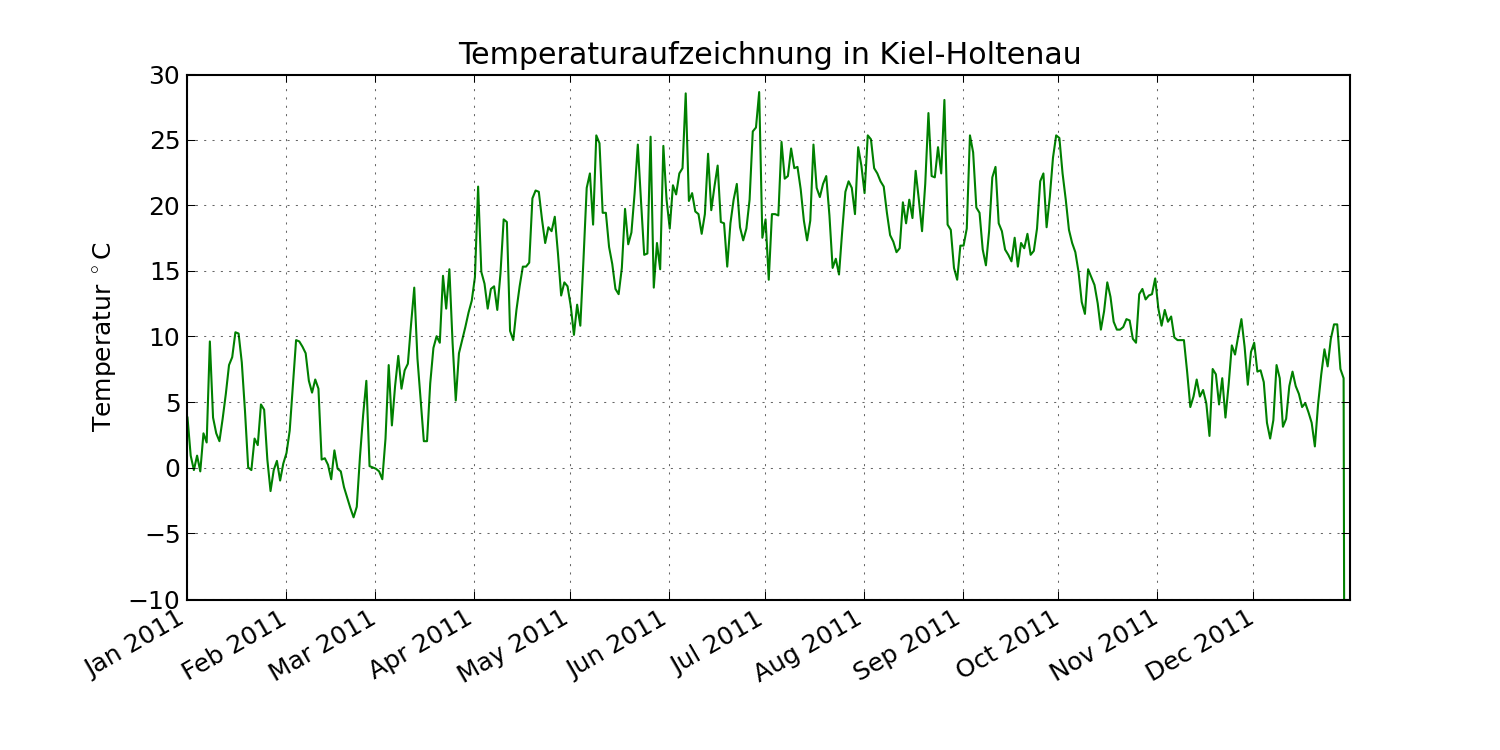
\includegraphics[width=.9\tw]{fig/03-Example-illustations/temperature-diagram_kiel}
  \caption{Darstellung einer Wertereihe der Art $f(x, t)$, Die Lufttemperatur im Jahresgang bei der Wetterstation Kiel-Holtenau.}
  \end{figure}
Darstellungen der Form $f(x,y)$:
\begin{itemize}
\item In 2D-Darstellungen wird der Messwert durch die Größe, Farbe oder Art der Symbole angezeigt. Ein Beipiel ist die Kennzeichnung von Epizentren durch Symbole, deren Größe proportional zur Magnitude ist. Statt einem kartesischen Koordinatensystem kann die Darstellung auch in anderen geographischen Projektionen oder in Polarkoordinaten erfolgen.
\item Konturplot (Isoliniendarstellung)
\item Einfärben von Bildpunkten. Eine Fotografie wird so dargestellt. Landkarten mit Höhenlinien sind eine Kombination dieser Darstellung mit einer Isoliniendarstellung.
\item 3D-Darstellungen von Oberflächen 
\item Darstellung in Polarkoordinaten: $f(r,\varphi)$
  \end{itemize}
Darstellungen der Form $ {\bf f}(x,y)$:
\begin{itemize}
\item
An den Orten $(x,y)$ werden Vektoren dargestellt, z.B. um Deformationen zu beschreiben.
\end{itemize}
Darstellungen der Form $f(x,y,z)$:
\begin{itemize}
\item Isooberflächen   
\item 3D-Plots mit Farbe, Größe oder Art der Symbole, die den Messwert $f$ anzeigen
\item Meistens werden 2D-Darstellungen der Messwerte auf ausgewählten, ebenen Schnitten bevorzugt. Beispiele sind Röntgenbilder.  
\item Es gibt Möglichkeiten der dreidimensionalen Darstellung, die meistens vor allem für die qualitative Bewertung sehr komplexer Datenstrukturen geeignet sind. 
  \end{itemize}
  
\noindent Darstellungen der Form $f(x,y,t)$: \begin{itemize}
\item Liegen flächenhafte Messungen als Funktion der Zeit vor, eignet sich die Visualisierung mit Hilfe von Filmen. Alternativ kann auch eine Folge von Bildern dargestellt werden.  
  \end{itemize}
Darstellung der Form $f(x,y,z,t)$:
\begin{itemize}
\item Derartige Messwerte - z.B. ein Dreikomponenten-Seismogramm - können auf einfachere Darstellungen zurückgeführt werden, indem die Komponenten des Seismogramms einzeln dargestellt werden. Es sind aber auch Projektionen der Partikelbewegung auf 3 senkrechte Ebenen möglich, wobei die Zeit farblich gekennzeichnet werden kann.
\end{itemize}
Weiterhin wurden spezielle Plots z.B. für die Darstellung von Herdflächenlösungen in Form sogenannter \textit{beachballs} entwickelt. 

\section{Bearbeitung der Signaldaten}
Im Folgenden werden Beispiele für die digitale Bearbeitung der Daten genannt.
\begin{itemize}
\item Trendkorrekturen, andere Korrekturen z.B. Korrektur von Zeitfehlern, Identifizierung und Entfernen von Ausreißern. 
\item Stapelung von Signalreihen
\item Detektion von Signal
\item Inter- und Extrapolation im Zeit- oder Ortsbereich
\item Approximation auch Komprimierung der Signalreihe
\item Resampling des Signalreihe
\item Korrelation : Korrelationsanalyse bei Vibroseismik, Kreuzkorrelation
\item Filterung und Wichtung in der Signalreihe
\item Transformationen (z.B. Fouriertransformation zur Berechnung von Frequenz- und Phasenpektren)
\end{itemize}

\section{Schätzung von Signalparametern}
Oft werden die bearbeiteten Daten nicht nur graphisch dargestellt, sondern es werden auch Signalparameter geschätzt, die interpretiert werden können oder als Input für Inversionen zur Verfügung stehen. Beispiele für Signalparameter sind:
\begin{itemize}
\item Signal-Rausch-Verhältnis, aber auch andere Qualitätsmaße
\item Frequenzspektren
\item Übertragunsfunktionen von Messgeräten und deren Korrektur
\item Herd-Zeit-Funktionen:(Abstrahlung im Herd), Wellenform des angeregten Signals
\item Schätzung einfacher Signalparameter wie Laufzeiten (Signaldetektion), Amplituden, Halbwertsbreiten etc., aber auch Schätzung von Streuamplituden durch Rückprojektion in einen Modellraum z.B. CMP-Stapelung
\item Schätzung von ARMA-Parametern, Poles and Zeros, Amplitude bzw. Phase einer bestimmten vorgegebenen Frequenz, Dämpfungsparamtern elastischer Wellen, Phasen- oder Gruppengeschwindigkeiten dispersiver Signale, Polarisationsparamter elastischer Wellen (z.B. Azimut, Einfallswinkel, Elliptizität), Eigenfrequenzen
\item Vorhersagen, Vorhersagefehler
\item Mustererkennung, Bestimmung von Ähnlichkeiten (z.B. Auto- und Kreuzkorrelation)
\item Slowness (Zeit-Frequenz-Analyse, f-k Analyse)
  \end{itemize}


\section{Modellierung/Inversion}
Während durch die Signalverarbeitung Parameter des Signals, z.B. seiner Form, geschätzt werden, werden durch Modellierung und Inversion Parameter eines phy\-sikalischen Modells geschätzt, mit denen die Messung möglichst gut erklärt werden kann. Ein Trend in einer P-Wellenlaufzeitmessung kann als Signal bezeichnet werden. Der Anstieg wäre dann ein Signalparameter der z.B. durch einen Halbraum mit einer bestimmten P-Wellengeschwindigkeit erklärt werden kann. Die P-Wellengeschwindigkeit ist der Parameter des physikalischen Modells - in diesem Fall eines Halbraums. Generell muss bei der Inversion zunächst eine geeignete Parametrisierung der relevanten gesteinsphysikalischen Parameter vorgenommen werden. Das geschieht allgemein durch Entwicklung nach Basisfunktionen, die ein-, zwei- oder auch dreidimensional sein können.  Weiter müssen für vorgegebene Parameter - Wichtungen der Basisfunktionen - theoretische Messwerte bestimmt werden können. Bei der Inversion werden dann durch eine möglichst effektive Strategie Parameter gesucht, die in einem gewissen Sinn optimal sind, beispielsweise die Fehlerquadratsumme zwischen gemessenen Werten und theoretischen Werten minimieren. Idealerweise werden noch mögliche Wertebereiche für die Parameter angegeben und Mehrdeutigkeiten untersucht.  

\section{Ablauf einer geophysikalischen Untersuchung}
Vor jeder geophysikalischen Untersuchung muss die Aufgabenstellung klar definiert werden. Die Messmethoden werden ausgewählt gegenüber der Aufgabenstellung und Genauigkeit. Sodann kann die Messungen durchgeführt werden.
Der zweite Schritt ist die Diskritisierung der Messergebnissen mit Hilfe der Analog-Digital-Umwandlung (A/D-Wandler) um eine diskritisierte Wertereihe (z.B. die Punktmessung der Schwerebeschlunigung). Anschliessend müssen die Daten organisiert werden - Lokationen müssen zugeordnet, und Zeiten ggf. korrogiert werden. Sind die Daten gemessen folgt im dritten Schritt bei einer geophysikalischen Untersuchung die Signalbearbeitung. Dabei können beispielhaft folgende Aktionen durchgeführt werden: 
\begin{itemize}
\item Visualisierung der Messgröße (Darstellung der Daten, Farbskala einführen)
\item Bearbeitung von Daten
\item Signalparameter abschätzen
\end{itemize}
Der nächste Schritt ist die Modellierung/Inversion der Daten (Physikalische Parameter, Vorwärtsmodellierung/Inversionsmodellierung). Im Anschluss können die Ergebnisse der geophysikalischen Untersuchung interpretiert werden.



\chapter{Begriffe und Definitionen}
\section{Kontinuierlich-diskret, analog-digital}
Das zu messende Feld ist in der Regel eine kontinierliche Funktion von Ort oder Zeit z.B. $x(t)$. Dabei ist $t$ die unabhängige und $x$ die abhängige Variable. Sowohl abhängige wie unabhängige Variablen sind kontinuierlich und können in einem bestimmten Wertebereich stufenlos jeden Wert annehmen. Durch Art der Messung (z.B. punktweise Messung) und Diskretisierung wird eine diskrete Wertereihe erhalten, wobei abhängige und unabhängige Variablen nur bestimmte, mit endlich vielen Ziffern darstellbare Werte annehmen können. Das Resultat ist die diskrete Wertereihe  $\{x_{i}\}=\{x_{1}, x_{2}, x_{3}, \dots, x_N\}$, wobei   $t_{i}=i\Delta t,~~ i =1,2, \dots, N,$ ist, mit einem Abtastschritt $\Delta t$. Nur diskrete Wertereihen sind für die digitale Bearbeitung mit Computern geeignet.  Die Funktion $x(t)=cos(\omega t)$ ist kontinuierlich bzgl. Zeit und Amplitude, die Wertereihe $\{ x_i \}= \{1,0,-1,0,1,0,-1,0\}$ ist dagegen diskret bzgl. Zeit und Amplitude. Die Spannung am Ausgang eines Seismometers ist kontinuierlich bzgl. Zeit und Amplitude, während die Spannung am Ausgang eines Computers zwar kontinuierlich bzgl. der Zeit ist, mitunter aber nur bestimmte Werte annehmen kann, also diskret bzgl. der Amplitude sein kann.     

Die Darstellung einer Messgröße kann analog oder digital erfolgen, d.h. in Form einer messbaren physikalischen Größe bzw. in Form von Ziffern. Beispiele für analoge Darstellungen sind graphische Darstellungen auf Bildschirm oder Papier, Seismogrammschriebe, wie Sie bis in die 70-iger Jahre des letzten Jahrhunderts üblich waren oder Aufzeichnungen auf Magnetband.  Die Anzeige der Uhrzeit kann analog oder digital erfolgen.  Die Auflistung von Wertereihen ist dagegen ein Beispiel für die digitale Darstellung. Die Schallplatte ist ein analoger Datenträger, eine CD oder DVD sind digtiale Datenträger. Die digitale Darstellung kann auch mittels Binärzahlen erfolgen. Beispiel: Binärzahl $1011=1\cdot 2^{3} + 0 \cdot 2^2 + 1 \cdot 2^1 + 1 \cdot 2^0 =$ die Dezimalzahl 11.

Es soll noch kurz auf andere Möglichkeiten der digitale Darstellung eingegangen werden. Um einen großen Wertebereich mit wenigen bits darzustellen, kann eine Verstärkung definiert werden. Ein Beispiel ist die 16-bit Datenerfassung die für die Darstellung von seismologischen Registrierungen verwendet worden ist. Dazu wurden ein bit für das Vorzeichen $V$, nur 11 bits für die binäre Darstellung eines Faktors $F$  und 4 bits für die binäre Darstellung des Exponent $E$ von 2 benötigt, durch den eine Verstärkung definiert wurde: $2^{E}$. Der dargestellte Wert ergibt sich dann nach $x = V*F*2^E$. Der minimale Wert von F ist  $F_{min}=0$, der maximale Werte ist $F_{max}=2^{11}-1 = 2047$. Für den minimalen Wert von $E$, $E_{min}=0$, ist die Verstärkung 1. Die maximale Verstärkung ergibt sich für $E_{max}=2^{4}-1=15$ und ist $2^{15}$. Der maximal darstellbare Wert ist dann  $x_{max}=(2^{11}-1) \cdot 2^{15} \approx 2^{26}$. Der minimale Wert hat ein negatives Vorzeichen und ist $x_{min} \approx = -2^{26}$. 

\subsection{Dynamik[umfang]}
Die Dynamik oder auch der Dynamikumfang ist das Verhältnis zwischen maximalem darstellbaren Betrag und minimalem darstellbaren Betrag größer Null. Sie wird berechnet nach  $20\log \frac{A_{max}}{A_{min}}$. Vorsicht: Mitunter wird auch ein Faktor 10 verwendet. Die  Einheit ist dB und steht für Dezibel. Dieses Kunstwort ist angelehnt an Graham Bell den Erfinder des Telefons.  Das Seismometer vom Typ STS2 kann maximale Geschwindigkeiten der Bodenbewegung bis ca. 0.1 m/s registrieren. Der kleinste Betrag is ca. 1 nm/s. Es ergibt sich ein Dynamikumfang von ca. 160 dB. Die oben dargestellte 16-bit Datenerfassung besitzt eine Dynamik von ca. 156 dB, eine Darstellung mittels Binärzahlen und 24 bit ergibt eine Dynamik von ca. 145 dB. Diese Datenerfassungen können also den Dynamikumfang des Seismometers nahezu abdecken. Offensichtlich muss die Verstärkung vor dem Analog-Digital-Wandler geeignet gewählt werden, so dass der interessierende Amplitudenbereich durch die Datenerfassung digitalisiert werden kann. Bei zu großer Verstärkung werden große Amplituden nicht mehr korrekt dargestellt(Clipping, Sättigung).  Bei zu geringer Verstärkung können kleine Amplituden nicht unterschieden werden. 

Zum Vergleich können wir die Dynamik eines seismologischen Papierschriebs abschätzen. Der maximale Ausschlag der Nadel könnte 15 cm betragen, der minimal noch wahrnehmbare Ausschlag 1 mm. Daraus ergibt sich eine Dynamik von ca. 43 dB. Da die Dynamik ein logarithmisches Maß ist, wird deutlich, dass für einen Papierschrieb das Verhälnis von maximal zu minimal darstellbarer Amplitude wesentlich kleiner ist als für digitale Datenerfassungen. 
 

\subsection{Auflösung} 
Neben der Dynamik ist die Auflösung ein wichtiger Parameter digitaler Darstellungen. Sie beschreibt die Differenz zwischen benachbarten darstellbaren Werten $\Delta x$. Für Binärzahlen ist sie 1. Für die besprochene 16-bit Darstellung ergibt sich: $(x + \Delta x)= V( F\pm 1)\cdot 2^E$. Die Auflösung ist also vom Exponenten abhängig und für größere Verstärkungen ist die Differenz zwischen benachbarten Werten größer. Die darzustellende Messgröße wird dann bei größeren Werten gröber diskretisiert. Generell muss je nach Aufgabenstellung ein Kompromiss zwischen Dynamik und Auflösung gefunden werden, da nur ein bestimmte Anzahl an bits für die Darstellung eines Wertes zur Verfügung steht. 

\subsection{least significant bit}
Ist ein Faktor, mit dem x multipliziert werden muss, um die Messgröße zu erhalten. Die Datenerfassung liefert zunächst nur einen einheitenlosen diskreten Wert. Erst durch Multiplikation mit dem least significant bit wird die Messgröße dargestellt. Zum Beispiel wird für seismologische Anwendungen das least signifcant bit einer 24-bit Datenerfassung oft 1.67 nm/s gewählt. 


\section{Deterministisch-stochastisch}
Um eine Wertereihe bearbeiten zu können, muss zunächst eine mathematische Beschreibung oder ein Modell für die Wertereihe aufgestellt werden. Dabei kann es sich um ein stochastisches oder ein deterministisches Modell handeln. Ein {\bf deterministisches} Modell kann durch digitale Werte oder durch einen funktionalen Zusammenhang beschrieben werden: z.B. ${x_i} = {0,1,1,0,-1,-1,0}$ oder $cos(\omega_0t)$. Deterministische Modell sind meistens vorhersagbar - siehe $cos(\omega_0t)$. Nur chaotische, deterministische Systeme sind nicht vorhersagbar. Ein {\bf stochastisches Modell } wird mit Hilfe von Wahrscheinlichkeitsdichteverteilungen beschrieben, d.h. es wird angegeben, mit welcher Wahrscheinlichkeit eine Zufallsgröße einen bestimmten Wert annimmt. Ein stochastisches Modell ist oft sehr praktisch. Z.B. zufällige Messfehler können so einfach beschrieben werden. Ein stochastisches Modell kann auch deterministische Komponenten enthalten. Ein Beispiel ist das Faltungsmodell der seismischen Spuren $y_i = w_i \star r_i + n_i$. Das wavelet $w_i$ wird als deterministisch angenommen, die Reflektivität des Untergrundes $r_i$ und das Rauschen $n_i$ als stochastisch. Interessant ist, dass hier für die eigentlich gesuchte Information, die Reflektivität, ein stochastisches Modell angenommen wird. 

Es muss von Fall zu Fall entschieden werden, ob ein deterministisches oder stochastisches Modell gewählt wird. Anhand des Modells der Wertereihe kann dann ein mathematischer Algorithmus für die digitale Signalbearbeitung erarbeitet werden. Eine deterministische bzw. eine stochastische Beschreibung können sowohl für das Nutz- wie das Störsignal geeignet sein. Ein 50 Hz Störsignal kann deterministisch beschrieben werden, störendes Rauschen würde man eher mit einem stochastischen Modell beschreiben. Wird mit Hilfe der Korrelation des seismischen Hintergrundrauschens (ambient noise) der Untergrund zwischen zwei seismischen Stationen untersucht, ist das Rauschen das Nutzsignal, für das ein stochastisches Modell angenommen wird. Für wiederholte Schweremessungen kann ein Modell angenommen werden, nach dem die tatsächliche Schwere eine deterministische Größe ist, die durch zufällige Messfehler überlagert wird. 

\subsection{Zufallsgröße x}
Die Wahrscheinlichkeit, dass die Zufallsgröße x den Wert s annimmt, wird durch die {\bf Verteilungsdichtefunktion} $p(s)$ bzw. durch die {\bf Verteilungsfunktion} $P(s)$ beschrieben. Die Verteilungsdichtefunktion kann eingipflig ({\bf unimodal}) oder mehrgifplig ({\bf multimodal}) zum Beispiel zweigipflig (bimodal) sein. Die Anzahl der Gipfel ist gleichbedeutend mit der Anzahl der Maxima. Außerdem kann die Verteilungsdichtefunktion symmetrisch oder unsymmetrisch um einen Wert s verteilt sein. Die Verteilungsfunktion wird definiert durch:\\ $P(s)=\int\limits_{-\infty}^s p(s')ds'$ , mit $p(-\infty)=p(\infty)=0$, $P(-\infty)=0$ und $P(\infty)=1$.\\
\underline {Bsp:} Gleichverteilung\\
$p(s)=\begin{cases}
  \frac{1}{2a},\text{für    }     m-a\leq s\leq m+a\\
 0, sonst 
\end{cases}$ \\für eine Verteilung der Breite 2a um den Mittelwert $m$. Die Verteilungsfunktion lautet dann \\ 
$P(s)=\begin{cases}
0,\text{für    } s<m-a\\
\frac{1}{2a},\text{für    }     m-a\leq s\leq m+a\\
1,\text{für    } s>m-a
\end{cases}$.
\\ \underline {Bsp:} Gaußsche Normalverteilung mit dem Mittelwert $m$ und der Standardabweichung $\sigma$. Die Zufallsgröße $x$ nimmt mit ca. 68\%-iger Wahrscheinlichkeit Werte zwischen $m-\sigma$ und $m+\sigma$ und mit ca. 95\%-iger Wahrscheinlichkeit Werte zwischen $m-2\sigma$ und $m+2\sigma$ an. Die Verteilungsdichtefunktion lautet:\\
$p(s)=\frac{1}{\sigma \sqrt{2\pi}}e^{-\frac{(s-m)^2}{2\sigma^2}}$ \\
und die dazugehörige Verteilungsfunktion\\  
$P(s)=\frac{1}{\sigma \sqrt{2\pi}}\int\limits_{-\infty}^s e^{{-\frac{(s'-m)^2}{2\sigma^2}}}ds'$.\\
Mit der Fehlerfunktion\\
$\mbox{erf}(x)=\frac{2}{\sqrt{\pi}}\int\limits_0^x e^{-x'^2}dx'$\\
folgt für die Verteilungsfunktion\\
$P(s) = \frac{1}{2}(\mbox{erf}(\frac{s-m}{\sqrt{2} \sigma}) + 1).$\\
Der Wertebereich der Fehlerfunktion ist $[-1,1]$ und der Wertebereich der Verteilungsfunktion ist wie immer $[0,1]$. Aufgrund der Symmetrie der Gaußschen Wahrscheinlichkeitsdichteverteilung gilt $P(m-s) = 1- P(m+s)$.


\subsection{Erwartungswert, Momente}
Eigenschaften von Zufallsgrößen können sehr einfach mit Hilfe des Erwartungswertes und statistischer Momente beschrieben werden.  $E[x]$, der {\bf Erwarungswert} der Zufallsgröße $x$, ist der Schwerpunkt der Wahrscheinlichkeitsdichtefunktion:\\
 $E[x] = \int\limits_{-\infty}^{\infty}sp(s)ds$.\\
Das erste Moment der Verteilungsdichtefunktion entspricht dem Erwartungswert: \\
$E[x]=m=m_1$.\\
Der Erwartungswert wird mit Hilfe der Wahrscheinlichkeitsdichtefunktion definiert. Die ist aber im Fall realer Wertereihen meist nicht bekannt. Deshalb muss der Erwarungswert anhand von Messungen - auch Realisierungen oder Stichproben $x_i$,   $i=1,\dots, N,$  geschätzt werden. Der Mittelwert der Messungen ist eine Schätzung für den Erwartungswert:\\
$\bar{x}=\hat{m_1}=\frac{1}{N}\sum \limits_{i=1}^N x_i$.
Dabei deutet das Dach an, dass es sich um eine Schätzung, in diesem Fall des ersten Moments, handelt. 

Für den Erwartungswert gelten einfache Rechenregeln:\\ 
 $E[x_1+x_2]=E[x_1]+E[x_2]$ und $E[a]=a$, falls $a$ eine deterministische Größe ist. Nimmt man für eine Messgröße ein Modell an, nach dem sie sich aus dem tatsächlichen Wert $a$ und zufälligem Rauschen $n_i$  zusammensetzt, $x_i = a + n_i$, so ist gilt für den Erwartungwert von $x_i$:\\
$E[x_i] = a + E[n_i]$.\\
 Ist der Erwartungswert von $n_i$ ungleich Null, kann auch durch Mittelung über viele Messwerte der tatsächliche Wert der gesuchten Größe nicht erhalten werden.

Es handelt sich um eine erwartungstreue (Englisch: {\bf unbiased}) Schätzung, wenn der Erwartunswert der Schätzung gleich der gesuchten Größe ist, z.B. $E[ \hat{m_1} ]= m_1$, wegen\\
$ E[\hat{m_1}] =\frac{1}{N}\sum \limits_{i=1}^N E[x_i] = m_1 $\\
ist das der Fall. Sonst würde es sich um eine nicht erwartungstreue (Englisch: {\bf biased}) Schätzung handeln. Dabei bedeutet bias Verzerrung. Allerdings kann erst für eine große Anzahl der Messungen die gesuchte Größe mit geringem Fehler geschätzt werden: 
 $\lim\limits_{N \to \infty}\frac{1}{N}\sum \limits_{i=1}^N x_i=E[x]=m_1$. 

Das {\bf zweite Moment} ist definiert durch:\\
$E[x^2]= \int\limits_{-\infty}^{\infty} s^2 p(s) ds=m_2$.\\
Es kann mittels\\
 $\bar x^2=\hat{m_2}=\frac{1}{N}\sum\limits_{i=1}^N x_i^2$\\
geschätzt werden. Das zweite zentrale Moment ist die Varianz. Sie ist definiert durch:\\
 $E[(x-E[x])^2]=\alpha_2=\sigma^2$, wobei $\sigma^2$ die Varianz und $\sigma$ die Standardabweichung sind. Die Schätzung kann mittels\\
$\hat{\alpha_2}=\frac{1}{N-1}\sum \limits_{i=1}^N (x_i - \bar x)^2 $\\
erfolgen. Auch für eine Schätzung kann die Varianz angegeben werden, z.B.\\
 $E[(\hat{m}-E[\hat{m}])^2].$\\
Für eine Gaußsche Zufallsgröße ist die Varianz für die Schätzung des Mittelwertes $\sigma^2/N$, die Standardabweichung der Schätzung des Mittelwertes ({\bf Standardfehler}) ist dann $\sigma/\sqrt{N}$. 

Wenn die Verzerrung und die Varianz einer Schätzung gegen Null gehen, falls N gegen Unendlich geht, handelt es sich um eine {\bf konsistente} Schätzung. Das ist im Fall der Schätzung des Mittelwertes der Fall.

Es können auch {\bf höhere Momente} definiert werden. Das n-te Moment ist:\\
$m_n=E[x^n]$\\
und es kann mittels\\
 $\hat{m_n}=\frac {1}{N} \sum\limits_{i=1}^N (x_i)^n$\\
geschätzt werden. 
Das {\bf n-te zentrale höhere Moment} ist:\\
 $\alpha _n=E[(x-E[x])^n]$\\
und seine Schätzung lautet:\\
 $\hat{\alpha_n}=\frac {1}{N-1} \sum\limits_{i=1}^N (x_i - \bar x)^n$. Die Eigenschaften einer Zufallsgröße können auch durch die Gesamtheit der Momente eindeutig beschrieben werden. \\
Mit Hilfe höherer Momente können die {\bf Schiefe} und die {\bf Kurtosis} bestimmt werden. Die Schiefe ist ein Maß für die Asymetrie der Verteilungsdichtefunktion:\\
$S=\frac {\alpha_3}{\sigma^3}=\frac {\alpha_3}{\alpha_2^{\frac{3}{2}}}$\\
und die Kurtosis ist ein Maß für die Abweichung von der Gaußverteilung:\\
$K=\frac {\alpha_4}{\sigma^4}=\frac {\alpha_4}{\alpha_2^2}$.\\
Für eine Gaußsche Zufallsgröße ist die Kurtosis 3.

Schiefe und Kurtosis können mit Hilfe der Schätzungen für die höheren zentralen Momente geschätzt werden:\\
 $\hat S=\frac {\hat{\alpha_3}}{\hat{\alpha}_2^{\frac{3}{2}}}$ 
bzw.\\
 $\hat K=\frac {\hat{\alpha_4}}{\hat{\alpha_2^2}}$.


\subsection{Stochastischer Prozess}

Eine Folge von Zufallsgrößen ${x_i}$ wird als stochastischer Prozess oder Zufallsprozess $\{x_i\}$ bezeichnet. Ein stochastischer Prozess kann auch eine kontinuierliche Funktion, z.B. der Zeit, sein: $x(t)$. Für jeden Index $i$ bzw. für jede Zeit $t$ existiert dann eine Zufallsgröße, deren Eigenschaften durch Wahrscheinlichkeitsdichtefunktionen beschrieben werden. Zum Beispiel kann für eine seismische Spur das Modell eines stochastischen Prozesses angenommen werden.  

Jede einzelne Spur (Messung) wird dann als Realisierung eines stochastischen Prozesses angesehen. 
Im Folgenden wird die Realisierung des stochastischen Prozesses $\{x_i\}$ mit dem Index $j$ beschrieben: $\{x_{ij}\}$ bzw. $x_j(t)$. Gibt es mehrere Realisierungen spricht man auch von einem Ensemble.

Der Erwartungswert eines stochastischen Prozesses kann mittels des Ensemble-Mittelwerts geschätzt werden, wenn die Anzahl der Realisierungen gegen Undendlich geht. Der Ensemble-Mittelwert von $x(t)$ für Zeit $t=t_1$ ist:\\ 
$\frac{1}{N}\sum\limits_{j=1}^{N}x_j(t_1)$.\\
Es kann auch über die Zeit gemittelt werden. Das ergibt den Zeit-Mittelwert für die Realisierung $j$:\\ 
$\frac{1}{2T}\int\limits_{-T}^{T}x_j(t)dt$.\\
Ensemble- und Zeit-Mittelwert müssen nicht, können aber, gleich sein. Vorraussetzung für die Gleichheit ist, dass der Erwartungswert eines stochastischen Prozesses zeitunabhängig ist. Man spricht von einem ergodischen Prozess oder {\bf Ergodizität}, wenn für $N \to \infty$ der Ensemble-Mittelwert gleich dem Zeit-Mittelwert ist. Sind alle Eigenschaften des stochastischen Prozesses zeitunabhängig, liegt (starke) {\bf Stationarität} vor.  

Sind alle Zufallsgrößen $x_i$  eine stochstischen Prozesses $\{x_i\}$ gaußverteilt, spricht man von einem {\bf Gaußprozess}.

Alle Zufallsgrößen eines {\bf iid-Prozesses} sind unabhängig und identisch verteilt (independent and identically distributed random numbers).

Im Fall eines Gaußschen iid-Prozesses sind alle Zufallsgrößen unabhängig und identisch gaußverteilt.

\newpage


\section{Signal-Rausch-Verhältnis (signal-to-noise ratio SNR)}
Das Signal-Rausch-Verhältnis dient der Einschätzung der Messqualität. Es wird aus den Daten abgeschätzt. Zunächst wird ein Modell angenommen:\\
$x_i=s_i + n_i.$
Dabei sind $x_i$ die untersuchte Wertereihe, $s_i$ das Nutzsignal und  $n_i$ ist störendes Rauschen.
Weiterhin soll gelten $E[s_i]=E[n_i]=0$ und $max\{|s_i|\}=|s|_{max}$ bzw. $max\{|n_i|\}=|n|_{max}$.\\
In Abhängigkeit des Modells gibt es verschiedene Möglichkeiten für die Abschätzung des SNR. Dabei ist entscheidend, welche Komponenten als deterministisch bzw. stochastisch angenommen werden.
\begin {itemize}
\item $s_i$ und $n_i$ sind deterministisch: $\frac {|s|_{max}}{|n|_{max}}$
\item $s_i$ deterministisch, $n_i$ stochastisch (iid ZP, gleichverteilt): $\frac {|s|_{max}}{|n|_{max}}$\\
\item $s_i$ deterministisch, $n_i$ stochastisch (gaußverteilt): $\frac {|s|_{max}}{\sigma_n}$\\
\item $s_i$ stochastisch, $n_i$ stochastisch (iid ZP, gaußverteilt): $\frac {\sigma_s}{\sigma_n}$\\
\end{itemize}
Für die Schätzung von $|s|_{max}, \sigma_s$ bzw. $|n|_{max}, \sigma_n$ wird ein Zeitfenster ausgesucht, in dem für das Rauschen  $n_i\approx 0$ gilt (Signalfenster) bzw. ein Rauschfenster in dem $s_i\approx 0$ ist. Überlagern sich Rauschen und Signal zeitlich ständig, müssen weitergehende Analysen durchgeführt werden.


\section{Energiesignal-Leistungssignal}
Ein transientes Signal, d.h. ein Signal endlicher zeitlicher Länge, wird auch als Energiesignal bezeichnet.  Für die Energie gilt $\int\limits_a^b |s(t)|^2 dt < \infty$.\\
Ein Leistungssignal besitzt eine unendliche zetliche Länge, d.h. es dauert länger an als Beobachtungsintervall lang ist. 
Es wird die Leistung in dem Zeitintervall $[a,b]$ bestimmt: $\frac{1}{b-a}\int\limits_a^b |s(t)|^2 dt$. Dabei bedeutet der Faktor $\frac{1}{b-a}$ eine Mittelung über die Zeit.



\chapter{Wiederholung}

\section{Faltung}
Kontinuierlich: 
\begin{equation}
x_1(t) \ast x_2(t)= \int\limits_{-\infty}^{\infty} x_1(t')x_2(t-t')dt',
\end{equation}
und diskret
\begin{equation}
x_{1i} \ast x_{2i} = \sum\limits_{j=-\infty}^{\infty} x_{1j} x_{2i-j}.
\end{equation}
Beschreibt Wirkung eines linearen Systems. $x_1(t)$: Input, $x_2(t)$: Impulsantwort des linearen Systems, $x_1(t) \ast x_2(t)$: Output.


\section{Korrelation (deterministisch)}
Gibt ein Maß für Ähnlichkeit von$ x_1(t)$ und $x_2(t)$\\
Kontinuierlich:
\begin{equation}
R_{x_1x_2}(t)= \int\limits_{-\infty}^{\infty} x_1(t')x_2(t'+t)dt',
\end{equation}
und diskret
\begin{equation}
R_{x_1x_2}(i) = \sum\limits_{j=-\infty}^{\infty} x_{1j} x_{2j+i}
\end{equation}
Bei der Korrelationsfunktion wird unterschieden in
\paragraph*{Kreuzkorrelationsfunktion} (KKF), Korrelation zweier verschiedener Funktionen und
\paragraph*{Autokorrelationsfunktion} (AKF), Korrelation der Funktion mit sich selbst.

\section{Fouriertransformation}
Kontinuierliche Funktion $x(t)$ wird als Reihe von harmonischen Funktionen unterschiedlicher Frequenz ausgedrückt. Kontinuierliches Spektrum (Spektraldichte) $X(\omega)$. Die Fouriertransformation in den $f$-Bereicht ist $F$, und $F^{-1}$ die Rücktransformation in den Zeitbereich:
\begin{align}
\textbf{F}\{x(t)\}  & = X(\omega) =\int\limits_{-\infty}^{\infty} x(t) e^{-i\omega t}dt\\
\textbf{F}^{-1}\{X(\omega)\} & = x(t) =\frac {1}{2\pi}\int\limits_{-\infty}^{\infty} X(\omega) e^{i\omega t}d\omega
\end{align}
Die Diskrete Fouriertransformation (DFT): diskrete Wertereihe $\{x_j\}$, diskretes Spektrum (Spektraldichte) $\{X_k\}, ~~ j,k=0,\dots,N-1$.
\begin{align}
DFT\{ x_j \} = X_k & =\sum\limits_{j=0}^{N-1}x_j e^{-i2\pi jk/N} \\
DFT^{-1}\{X_k\} = x_j & =\frac{1}{N} \sum\limits_{k=0}^{N-1}X_k e^{-2\pi jk/N}
\end{align}
Dabei ist $\{x_j\}$,$\{X_k\}$ periodisch, Periode: $N$\\

\subsection{Darstellung des Spektrums}
{\color{red} MUSS ÜBERARBEITET WERDEN!!!}
Für ein diskretes Signal gilt das maximal Frequenzen bis zur Nyquistfrequenz abgetastet werden können. Die Nyquistfrequenz ist definiert als
\begin{equation}
f_{Ny} = \frac {1} {2 \Delta t N}
\end{equation}
und der Abtastschritt
\[
\Delta t =\frac{1}{\Delta t N} = \frac{1}{T}
\]
Die diskrete Fourier Transformation (DFT) berechnet das Spektrum $X_k$ für eine diskrete Signalreihe, bei der gilt $\omega_k= k \Delta \omega, k=0,\dots, N-1$ im Intervall $[0,2\omega_{Ny}]$. Für die Nyquistfrequenz gilt $\omega_{Ny} = \frac {\pi} {\Delta t N}$ und für den Abtastschritt im Frequenzbereich bzgl. der Kreisfrequenz gilt $\Delta\omega=\frac{2\pi}{\Delta t N} = \frac{2\pi}{T}$ , wobei $T$ die Länge des Beobachtungsintervalls im Zeitbereich ist. Bezüglich der Frequenz wird das Spektrum $X_k$ für die Frequenzen  $f_k, k=0,\dots, N-1$ im Intervall $[0,2f_{Ny}]$ berechnet.\\\\
Der Abtastschritt im Frequenzbereich bestimmt die Auflösung der DFT. Zwei Frequenzen $f_1$ und $f_2$ können unterschieden werden, wenn der Betrag ihrer Differenz größer als $ \Delta f$ ist. D.h. für die Länge der Wertereihe im Zeitbereich muss  gelten
\[
N \ge \frac{1}{\Delta t | f_1 - f_2 |}.
\]
Eine längeres Signal hat einen kleineren Abtastschritt im Frequenzbereich und eine höhere Auflösung zur Folge. Dies nennt man Unschärferelation.\\\\
Die Darstellung des Spektrums erfolgt für reelle Wertereihen im Intervall $[0,f_{Ny}]$, da das Spektrum bezüglich $f_{Ny}$ symmetrisch ist. Um die nicht dargestellten Frequenzen zu berücksichtigen, kann statt dem Amplitudenspektrum $|X_k|$ der doppelte Wert $2|X_k|$ dargestellt werden.\\\\
Für das Phasenspektrum gilt:
\[
X_k= |X_k|e^{i\varphi_k},
\]
wobei $\varphi_k$ das Phasenspektrum ist, für das gilt:
\[
\varphi_k = \arctan \left(\frac{Im\{X_k\}}{Re\{X_k\}}\right) + 2n\pi
\]
{\small Dabei ist $n \in \mathbb{G}$}\\\\
Das bedeutet dass das Phasenspektrum aufgrund der harmonischen Schwingungen mehrdeutig ist. Deshalb wird entweder die Phase für verschiedene $n$ berechnet und dargestellt oder es wird für jedes $k$ ein $n$ gefunden, so dass der Betrag der Phasendifferenz für aufeinanderfolgende $k$ minimal ist. Man sagt, die Phase wird aufgerollt. Da eine Zeitverschiebung des Signals einen linearen Trend in der Phase erzeugt, kann der Zeitpunkt Null so verschoben werden, dass die Phase einen minimalen Trend zeigt. Z.B. kann der Schwerpunkt des Signals als Zeitpunkt Null gewählt werden, um einen linearen Trend in der Phase zu minimieren.

\subsubsection*{Verwendung von Zeitfenstern}
Ein transientes Signal ist ein Rechteckfenster in dem dass Signal vollständig enthalten ist.\\
Das Leistungssignal: Die Enden werden herunter gewichtet, um Unstetigkeiten an den Enden des Beobachtungsinvervalls zu dämfen. Das Signal wird mit einem \textit{Taper} multipliziert. Beispiele für häufig verwendete Zeitfenster sind:
\begin{itemize}
\item Hamming-Fenster (nach Richard Hamming)
\[
0.54+0.46\cos \left(\frac{2\pi j}{N} \right)
\]
{\small Wobei $j=-\frac{N}{2},\dots, \frac{N}{2}-1$}
\item Hanning-Fenster (von Hann)
\[
\frac{1}{2}\left(1+\cos\left(\frac{2\pi j}{N}\right)\right)
\]
{\small Wobei $j=-\frac{N}{2},\dots, \frac{N}{2}-1$}
\end{itemize}
Es können auch nur die Enden des Zeitfensters mit einem Hanning Fenster gewichtet werden.
Das Powerspektrum eines stochastischen, stationären Signals wird geschätzt, indem es für überlappende Segmente einzeln berechnet und dann gemittelt wird. Zuvor werden die Segmente jeweils mit einem Zeitfenster multipiziert.

\subsection{Mehrdimensionale Fourier Transformation}
Fourier Transformation bezüglich Zeit
\[
f(t) \xrightarrow {\bf F} F(\omega)
\]
Fourier Transformation bezüglich Ort
\[
f(x) \xrightarrow {\bf F} F(k)
\]
Wellenzahlbereich beträgt 
\[
k=\frac{2\pi}{\lambda}.
\]
{\small Dabei ist $k$ die Wellenzahl und $\lambda$ die Wellenlänge.}
Vergleiche: $ \omega =\frac{2\pi}{T}$.

\subsubsection{2-Dimensionale Fourier Transformation}
Beispiele für 2-dimensionale Fourier Transformationen

\begin{align}
F(k_x,k_y) = &\iint_{-\infty}^\infty f(x,y)e^{-i(k_xx+k_yy)} dx dy\\
f(x,y)= &\frac{1}{4\pi^2} \iint_{-\infty}^\infty F(k_x,k_y)e^{i(k_xx+k_yy)} dk_x dk_y\\
F(k,\omega)= & \iint_{-\infty}^\infty f(x,t)e^{-i(kx+\omega t)} dx dt\\
f(x,t)=&\frac{1}{4\pi^2}\ \iint_{-\infty}^\infty F(k,\omega)e^{i(kx+\omega t)} dk d\omega
\end{align}

\subsubsection{3-Dimensionale Fourier Transformation}
Beispiele für 3-dimensionale Fourier Transformationen

\begin{align}
F(k_x,k_y,\omega)= & \iiint_{-\infty}^\infty f(x,y,t)e^{-i(k_xx+k_yy+\omega t)} dx dy dt\\
f(x,y,t)= & \frac{1}{8\pi^3} \iiint_{-\infty}^\infty F(k_x,k_y,\omega))e^{i(k_xx+k_yy+\omega t)} dk_x dk_y d\omega
\end{align}

\subsection{Sätze}

\paragraph{Umkehrsatz}
\begin{equation}
\textbf{F} \{X(\omega)\}=2\pi x(-t)
\end{equation}
Vergleiche:
\[
{\bf F} \{x(t)\}=X(\omega) \mbox{ und } {\bf F}^{-1}\{X(\omega)\}=x(t)
\]


\paragraph{Verschiebungssatz}
\begin{equation}
\textbf{F} = \{x(t+b)\}=e^{ib\omega}X(\omega)
\end{equation}
$e^{ib\omega}$ ändert Phase nicht das Amplitudenspektrum, ein Linearer Trend wird zur Phase addiert.


\paragraph{Differentiationssatz}
\begin{equation}
\textbf{F}\{x^\prime(t)\}=i\omega X(\omega)
\end{equation}
Der Faktor $i \omega$ bewirkt eine Phasenverschiebung um $\mbox{sgn}(\omega) 90^\circ$ und hohe Frequenzen werden verstärkt.

\paragraph{Integrationssatz}
\begin{equation}
\textbf{F} \{\int\limits_{-\infty}^{t} x(t')dt'\}=\frac{1}{i\omega} X(\omega)
\end{equation}
Der Faktor $1/i\omega$ bewirkt eine Phasenverschiebung um $-\mbox{sgn}(\omega) 90^\circ$ und tiefe Frequenzen werden verstärkt.

\paragraph{Faltungssatz} 
\begin{equation}
\textbf{F} \{x_1(t) \ast x_2(t)\}= X_1(\omega) X_2(\omega)
\end{equation}
Faltung im Zeitbereich bedeutet Multiplikation im Frequenzbereich. Umgekehrt entspricht auch eine Multiplikation im Zeitbereich bis auf einen konstanten Faktor einer Faltung der Spektren im Frequenzbereich.

\paragraph{Korrelationssatz}
\begin{equation}
\textbf{F} \{\rho_{x_1x_2}(t)\}= X_1^\ast(\omega) X_2(\omega)
\end{equation}
Beachte den Unterschied zum Faltungssatz. Wie beim Faltungssatz werden die Amplitudenspektren multipliziert. Die Phasenspektren werden aber subtrahiert, bei der Faltung addiert.

\paragraph{Rayleigh-Theorem}
\begin{equation}
\int\limits_{-\infty}^{\infty} | x(t) |^2 dt = \frac{1}{2\pi} \int\limits_{-\infty}^{\infty} | X(\omega)|^2 d\omega
\end{equation}
Power im Zeitbereich = $\frac{1}{2\pi}$ Power im Frequenzbereich.

\paragraph{Ähnlichkeitssatz}
\begin{equation}
{\bf F} \{x(at)\}= \frac{1}{a} X\left(\frac{\omega}{a}\right)
\end{equation}
Stauchung einer Funktion bzgl. Zeit im Zeitbereich entspricht Dehnung des Spektrums bzgl. Frequenz im Frequenzbereich.


\section{Aliasing}
Aliasing tritt auf, wenn der Abtastschritt, $\Delta t$ zu klein gewählt ist, dadurch wird das Spektrum verfälscht.
\begin{itemize}
\item Es werden mindestens zwei Ableitungen für die kürzeste Periode benötigt
\[
\frac{1}{f_{max}}
\]
\item Höchste Frequenz, die mit bestimmten Abtastschritt wiedergegeben werden kann
\[
\frac{1}{2\Delta t} \rightarrow \mbox{Nyquist-Theorem}
\]
\item Nyquistfrequenz
\[
f_{Ny}=\frac{1}{2 \Delta t}
\]
\end {itemize}
Wie Aliasing des Signal vermieden werden kann:
\begin{itemize}
\item $\Delta t$ so klein wählen, dass
\[
f_{max} < \frac {1}{2\Delta t}
\]
\item Antialiasingfilter: analoger Filter vor Digitalisierung der Messgröße.
\item In der Praxis wird \textbf{drei- bis vierfaches} oversampling empfohlen, so dass
\[
f_{Ny}\approx 4-5 f_{max}.
\]
\end {itemize}

\chapter{Vorbereitende Datenbearbeitung}

\section{Prüfen der Datenqualität}
Vor einer Analyse der Messreihen muss immer eine kritische Bewertung der Datenqualität erfolgen. Wenn nötig, müssen Korrekturen vorgenommen werden oder Messdaten aufgrund mangelnder Qualität verworfen werden. Die Bewertung der Datenqualität erfolgt meist visuell. Eine automatische Kontrolle ist jedoch wünschenswert. Die Kriterien für die Überprüfung der Datenqualität sind sehr stark von dem Untersuchungsziel abhängig. Es muss z.B. gefragt werden:
\begin{itemize}
\item
Ist die Abtastung adäquat? Die Abtastrate darf nicht zu gering und sollte nicht zu hoch sein. Eine äquidistante Abtastung ist generell zu bevorzugen. Liegt sie nicht vor, kann sie z.B. durch Interpolation hergestellt werden.
\item
Ändert sich die Qualität der Messreihe? Mitunter müssen fehlerhafte Segmente identifiziert und beseitigt werden. Es kann z.B. vorkommen, dass für ein bestimmtes Messintervall fehlerhafte Messwerte oder konstante Messwerte oder Datenlücken vorliegen. Oft sind auch nur einzelne Werte fehlerhaft (Ausreißer). Sie müssen identifiziert und beseitigt werden.
\item
Wesentlich ist, das SNR zu prüfen. Ist das Signal überhaupt zu erkennen? Lohnt sich eine Bearbeitung der Daten?
\item
Oft gibt es spezielle Fragestellungen. Z.B.: ist die Polarität korrekt? Ist die Orientierung der Komponenten korrekt? Sind die Amplituden korrekt? Gibt es Zeitfehler? Zeitfehler sind oft schwer zu erkennen, können aber z.B. durch den Drift der internen Uhr (Beispiel Ozeanbodenseismometer) auftreten. Mitunter hilft ein Vergleich von markanten Signalen, die an der zu untersuchenden und einer Referenzstation registriert worden sind, um Zeitfehler zu erkennen. Auch die mittels ambient noise berechnete Greensfunktion kann für das Erkennen der Zeitdrift verwendet werden. Relative Laufzeiten sind unabhängig von der Fehlern in der absoluten Zeit und können verwendet werden, falls eine zuverlässige Korrektur des Zeitfehlers nicht möglich ist.    
\end{itemize}
Eine Verbesserung der Datenqualität kann mitunter durch einfaches Entfernen fehlerhafter Daten erfolgen, mitunter muss ein anspruchsvolle und optimierte Signalverarbeitung erfolgen. 

\section{Einfache Transformationen}

\section{Trendbestimmung und -korrektur}
Einer der ersten Schritte der Signalverarbeitung ist die Bestimmung des Trends. Der Trend kann sowohl Nutz- wie Störsignal sein. Um ihn bestimmen zu können, wird ein Modell angenommen:
\[
x_i=m_i + y_i
\]
Dabei ist $x_i$ die betrachtete Wertereihe, die sich aus dem Trend $m_i$ und einem überlagerten Signal $y_i$ zusammensetzt. Im Fall der Seismik oder Seismologie ist ${y_i}$ das Nutzsignal und der Trend soll bestimmt und beseitig (korrigiert) werden. Für die Entwickung der Bevölkerungszahl oder für Börsenkurse ist ${m_i}$ das interessierende Phänomen und ${y_i}$ würde als Rauschen bezeichnet werden können.\\\\
Eine Möglichkeit den Trend zu bestimmen ist, ein Modell für den Trend anzunehmen und dessen Parameter zu schätzen. Oft wird für den Trend das Modell eines Polynoms gewählt:
\[
m_i(a_j)=a_0+ a_1t_i+a_2t_i^2+\dots = \sum\limits_{j=0}^{q} a_j t_i^j
\]
Dbei sind ${a_j}$ die Koeffizienten des Polynoms, welche nach der Methode der kleinsten Quadrate bestimmt werden können. Dabei wird die Fehlerquadratsumme $E$ minimiert:
\[
E=\sum\limits_{i=0}^N (x_i -m_i)^2 \rightarrow \mbox{Min.}
\]
D.h. für die Koeffizienten soll gelten:
\[
\frac{\partial E}{\partial a_k}\stackrel{!}{=}0
\]
Diese Bedingung liefer ein lineares Gleichungssystem zur Lösung der Parameter. Die Lösung des Gleichungssystems liefert dann die Schätzungen $\hat{a_k}$, mit denen der Trend des Signals gesschätzen werden kann: $m_i(\hat a_k)$. Die trendkorrigierte Wertereihe ist dann:
\[
\hat{y_i}=x_i-m_i(\hat a_k)
\]
Zu beachten ist, dass das Zeitfenster und die Ordnung $q$ des Polynoms geeignet gewählt werden müssen. Die Ordung $q$ sollte möglichst klein (z.B. 1.-Ordnung für einen linearen Trend) gewählt und wenn nötig schrittweise erhöht werden. Die Ordnung muss so klein sein, dass das $m(\hat a_k)$ nicht Anteile von ${y_i}$ enthält. Das Zeitfenster sollte eher zu lang als zu kurz gewählt werden. Möglicherweise kann der Trend auch in einem Zeitfenster vor dem Einsetzen eines Signals bestimmt werden.\\\\

\subsection{Moving Average}
Der Trend kann auch mittels Filterung oder eines gleitendes Mittels, (eng. \textsl{Moving Average}, MA) bestimmt werden.\\\\
Ein \textit{akausales}, zweiseitiges Fenster hat eine Länge von $2q + 1$. Dabei wird auch auf zukünftige Werte zugegriffen, die Bearbeitung kann also nur \textbf{offline} erfolgen.
\begin{equation}
\hat{m_i}=(2q+1)^{-1}\sum\limits_{j=-q}^q x_{i-j}
\end{equation}
Für ein \textit{kausales}, ein einseitiges gleitendes Fenster wird nur auf aktuelle und vergangene Werte zugegriffen. Diese Variante ist geeignet für die Bestimmung des Trends in Echtzeit (\textbf{online}). Allerdings führt dies zu einer Phasenverschiebung der Signale.
\begin{equation}
\hat{m_i}=(q+1)^{-1}\sum\limits_{j=0}^q x_{i-j}
\end{equation}

Das gleitende Mittel kann auch rekursiv bestimmt werden
\begin{equation}
\hat m_i=(q+1)^{-1} x_i +  \hat m_{i-1}-(q+1)^{-1} x_{i-1-q}
\end{equation}
Dabei ist $x_i$ der aktuelle Wert in der Signalreihe. Setzt man $x_{i-1-q}\stackrel{!}{=}\hat m_{i-1}$ werden nur $\hat m_{i-1}$ und $x_i$ benötigt
\begin{equation}
\hat{m_i}= \alpha x_i + (1-\alpha) \hat m_{i-1}
\end{equation}
Dabei ist $\alpha = (q+1)^{-1}$\\
Diese Näherung ist sehr einfach zu berechnen. Sie ist nicht exakt, aber oft ausreichend.\\\\
In einem gleitenden Fenster können statt dem Mittelwert auch Quartile geschätzt werden. Quantile $Q_p$ ist der Wert $s$, für den die Verteilungsfunktion $\underline P(s)=p$ ist. $Q_{0.5}$ ist der Median, $Q_{0.25},Q_{0.5},Q_{0.75}$ sind Quartile der Verteilung.

\section{Saisonale Komponenten}
Interessant ist auch der Fall, in dem eine periodischer Anteil (saisonale Komponente) bestimmt werden und möglicherweise beseitigt werden sollen.
\[
x_i=s_i + y_i
\]
Dabei ist $x_i$: Wertereihe, $s_i$: saisonale Komponente (z.B. Jahres-, Tagesgang, 60 Hz Stromnetz oder Milankovic-Zyklen) und $y_i$: Signalreihe.\\\\
Mögliche Methoden um die Saisonale Komponente Im Signal zu erfassen:

\begin{enumerate}
\item Kann man die Signalreiehe Differenzieren oder Filtern? Hilft es das Spektrum zu berechnen, um Frequenzen der saisonalen Komponente zu erkennen.

\item Moving Average $d$, die Periode von $s_i$ ist bekannt. Ein $q$ wählen, so dass $d=2q+1$\\

\item Ein Modell für saisonale Komponenten annehmen, Parameter bestimmen, $\hat s_i$ schätzen und von $x_i$ abziehen.

\paragraph{Beispiel} Externe Messung einer Störgröße $p_i$. Als Modell kann im einfachsten Fall $s_i=f(p_i) = ap_i$ angenommen und $a$ kann nach der Methode der kleinsten Quadrate bestimmt werden. Hier kann $x_i$ z.B. eine kontinuierliche Schweremessung und $p_i$ eine Messung des Luftdrucks sein. 

\paragraph{Beispiel} Ein etwas komplizierteres Modell ist die Überlagerung von Cosinus-Funktionen verschiedener Frequenz.
\[
s_i=\sum\limits_{j=0}^N a_j \cos(w_jt_i+\varphi_j)
\]
Wobei $a_j$,$\varphi_j$: unbekannt; $\omega_j$: bekannt\\
Mithilfe des Additionstheorems und Lösung dessen können die unbekannten Schwingungen identifiziert werden.
\[
s_i=\sum\limits_{j=0}^N a_j (\cos(w_jt_i)\cos(\varphi_j) - \sin(w_jt_i) \sin(\varphi_j))
\]
Wobei die Phase der Signale $\phi$ unbekannt ist\\
Die Gleichung kann umformuliert werden zu:
\[
s_i=\sum\limits_k c_k b_{ki}
\]
Dabei ist
\[
b_{ki}=
\begin{pmatrix}
\cos(\omega_1t_i)\\
\vdots \\
\cos(\omega_qt_i \\
-\sin(\omega_1t_i)\\
\vdots \\
-\sin(\omega_qt_i
\end{pmatrix}
; c_k=
\begin{pmatrix} 
a_1 \cos(\varphi_1)\\
a_2 \cos(\varphi_2)\\
\vdots\\
a_1 \sin(\varphi_1) \\
a_2 \sin(\varphi_2)
\end{pmatrix}
\]
Mithilfer der Methode der Kleinsten Quadrate Lösen wir:
\[
E = \sum\limits_i (x_i- \sum\limits_j c_j b_{ji})^2
\]
zu
\[
\sum\limits_i x_i b_{ki} = \sum\limits_j c_j\sum\limits_i b_{ji}b_{ki}
\]
Rechte Seite einer Bestimmungsgleichung ist die Projektion der Messwerte auf Basisfunktionen
Weiter gilt:
\[
a_j=(c_j^2+c_{j+a}^2)^{0.5}, \varphi_j=\arctan(\frac{c_{j+a}}{c_j})
\]

\paragraph{Beispiel} $s_i=a \cos(\omega t + \varphi)$; wobei zusätzlich zu $a$ und $\varphi$ auch die Frequenz $\omega$ unbekannt ist. Durch die unbekannte Frequenz wird das Problem nicht-linear. Es müssen Methoden der nicht-lineare Optimierung genutzt werden, um die Parameter $\omega, a$ und $\varphi$ zu bestimmen.
\end{enumerate}

\section{Resampling einer Signalreihe}
Will man den Abtastschritt (eng. \textsl{Samplingrate}) einer schon aufgezeichneten Zeitereihe ändern kann die Interpolation des Signals im Frequenz oder Zeitbereich durchgeführt werden.

\subsection{Interpolation im Zeitbereich}
Im Zeitbereich kann der Abtastschritt einer diskreten Signalreihe durch harmonisch überlagernde $Sinc$ Funktionen erhöht werden.
\begin{equation}
x(t) = \sum_{j=0}^{N-1} x(j \Delta t) \, \mbox{sinc} \left(\omega_{Ny}(t-{t_j}\right)
\end{equation}
Die Superposition der Sinc Funktionen ist jeweils um $t_j$ verschoben und je mit der gemessenen Amplitude $x(j\Delta t)$ gewichtet.

\begin{figure}[h!]
\centering
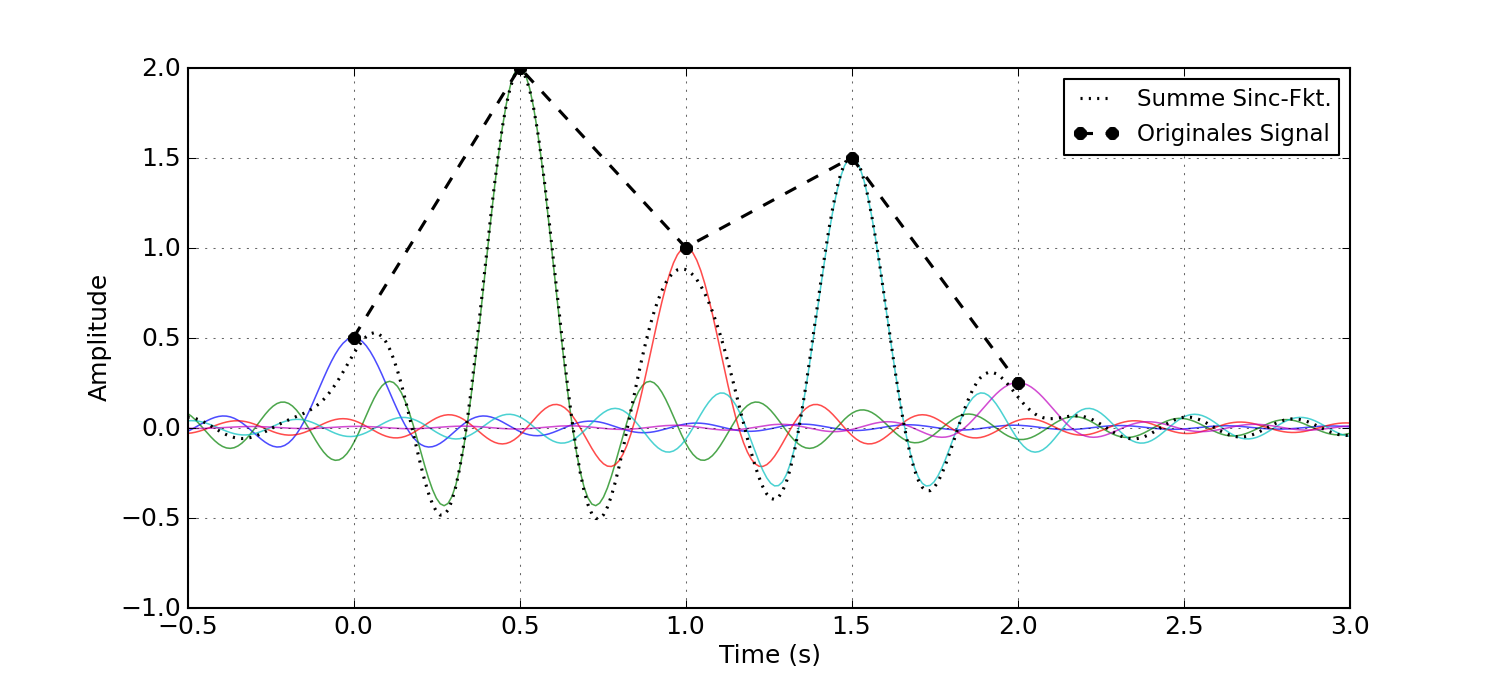
\includegraphics[width=.9\tw]{fig/04-Daten/interpolation_sinc.png}
\caption{Interpolation im Zeitbereich durch gewichtete und überlagernde Sinc Funktionen.}
\end{figure}


\chapter{Stapelung von Signalen}
Das Stapeln von Signalereihen wird genutzt um ein besseres Signal zu Rausch Verhältnis (eng. \textsl{Signal-to-Noise Ratio}) des gewünschten Signals zu bekommen als auch bei der räumlichen Analyse von Signalen.
Die Stapelung der Signalreihen wird benutzt bei:
\begin{itemize}
\item Wiederholter Anregung des Input Signals\\
Z.B. in der Hammerschlagseismik oder Ultraschall.
\item Bündelung von Geophonen ($\rightarrow$ \textit{Geophone Group Interval})
\item Gruppierung von Quellen\\
Z.B. bei der Vibroseismik.
\item Stapelung von Seismogrammen\\
Wie bei der CMP Stapelung, reflektierte Wellen werden nach der \textit{Normal-Move-Out} (NMO) Korrektur gestapelt.
\end{itemize}

\section{Beispiele der Stapelung}
\subsubsection*{Beispiel}
Überlagerung zweier Signale mit gleicher Frequenz $\omega_0$, aber unterschiedlicher Phase.  Das ist ein einfaches Beispiel für eine Stapelung mit $t_i\not= 0$ und $n_i=0$. Die zwei Signale sind:
\begin{align*}
s_1(t) & =\cos(\omega_0 t+\varphi_1)\\
s_2(t) & =\cos(\omega_0 t+\varphi_2).
\end{align*}
Mit dem Additionstheorem ergibt die Überlagerung:
\begin{equation}
s_1(t)+s_2(t)=2 \cos \left(\omega_0 t + \frac {\varphi_1 + \varphi_2}{2}\right)\, \cos\left(\frac {\varphi_1 - \varphi_2}{2}\right).
\end{equation}
Das bedeutet die Frequenz ändert sich nicht. Die Phasenverschiebung wird gemittelt und es ergibt sich ein zeitunabhängiger Wichtungsfaktor, der von der Phasendifferenz abhängt. Für $\varphi_1-\varphi_2= \pi $ löschen sich die Signale gegenseitig aus.\\\\
Für eine Phasenverschiebung von $|\varphi_1-\varphi_2|\le \frac{\pi}{2}$ ($\Delta\varphi = \frac{\lambda}{4}$) gilt für den Wichtungsfaktor $\cos \left(\frac{\varphi_1-\varphi_2}{2} \right)\ge 0.7071$ und es liegt konstruktive Interferenz vor.\\ 

\subsubsection*{Beispiel}
Überlagerung zweier Signale mit unterschiedlicher Frequenz:
\begin{align*}
s_1(t) & = \cos(\omega_1 t)\\
s_2(t) &= \cos(\omega_2 t)
\end{align*}
Mit dem Additionstheorem folgt:
\begin{equation}
s_1(t)+s_2(t)= 2 \cos \left(\frac{\omega_1+\omega_2}{2}t\right)\, \cos \left(\frac{\omega_1-\omega_2}{2}t\right).
\end{equation}

Es ergibt sich eine Schwebung mit einer hochfrequenten Trägerfrequenz $\frac{\omega_1+\omega_2}{2}$ und einer niederfrequenten Amplitudenmodulation mit der Frequenz $f_A = \frac{1}{2\pi}\frac{\omega_1-\omega_2}{2}$. Interessant ist, dass zu den Zeitpunkten $\frac{n}{2f_A}+\frac{1}{4f_A}$ mit $n \in \mathbb{G}$ ein Phasensprung auftritt. Die Maxima der Einhüllenden sind ebenfalls $\frac{1}{2f_A}$ entfernt. Beachte: wird eine Fourieranalyse von diesem Signal gemacht, treten nur die Frequenzen $\omega_1$ und $\omega_2$ auf. Die Formulierung mit amplitudenmodulierter Trägerfrequenz ist jediglich äquivalent.\\ 

\subsubsection*{Beispiel}
Ein Signal soll zwei Frequenzen $\omega_1$ und $\omega_2$ enthalten: $s(t) = \cos (\omega_1t) + \cos(\omega_2t)$. Betrachtet wird die Überlagerung zweier zeitverschobener Signale:
\begin{align*}
s_1(t) &=s(t+t_1)\\
s_2(t) &=s(t+t_2)
\end{align*}

Mit dem Additionstheorem folgt:
\begin{multline}
s_1(t)+s_2(t)= 2 \cos \left(\omega_1 t +\omega_1\frac{t_1+t_2}{2}\right)\, \cos \left(\omega_1\frac{t_1-t_2}{2}\right)\\
+2 \cos \left(\omega_2 t +\omega_2\frac{t_1+t_2}{2}\right)\, \cos\left(\omega_2\frac{t_1-t_2}{2}\right).
\end{multline}

\begin{itemize}
\item Die Frequenzen $\omega_1$ und $\omega_2$ bleiben erhalten.
\item $\cos (\omega_1\frac{t_1-t_2}{2})=f_1$ und $ \cos(\omega_2\frac{t_1-t_2}{2})=f_2$ sind zeitunabhängige Wichtungsfaktoren für die beiden Frequenzen.
\item Für $\omega_1<\omega_2$ ist $f_1>f_2$, d.h. die Stapelung ist ein Tiefpass. Die Bedingung für konstruktive Interferenz ist für tiefe Frequenzen eher erfüllt als für hohe Frequenzen. 
\end{itemize}

\section{Beamforming}
Bei Beamforming sucht man die richtige Wellenzahlvektor $\vec{k}$ der einfallenden Erdbebenwelle in ein Array von Seismometern. Dabei wird die Stappelung von vielen Seismogrammen benutzt um den Wellenzahlvektor der einfallenden seismischen Welle zu bestimmen.\\
Ein Seismogramm $u(x,y,t)$ kann als Funktion der Zeit und des Ortes plus Rauschen dargestellt werden:
\begin{equation}
u(x,y,t) = s(t-t_{j})+m(x_{j},y_{j},t)
\end{equation}
Dabei ist $s(t-t_{j})$ das zeitverschobene Signal um $t_j$ und $m(x_{j},y_{j},t)$ das ortsabhängige gleichverteilte Rauschen.\\
Nun werden viele Slowness Vektoren berechnet. Für die wahre Slowness $\vec{p}$ gilt: 
\[
\vec{p} \approx \hat{\vec{p}}
\]
So ist die Zeitverschiebung ist der Station $j$ für einen Slowness Vektor $\hat{\vec{p}}$ relativ zum Zentrum des Arrays $\vec{r}$:
\begin{equation}
\hat{t}_{j}=\hat{\vec{p}} \vec{r}
\end{equation}
Durch Summieren für eine bestimmte Slowness $\hat{\vec{p}}$ über alle Stationen wird ein Beam $b(t)$ erzeugt:
\begin{equation}
 b(t) = \sum_{j=1}^{n} u( x_j,y_j,t+t_j)
\end{equation}
Wobei $j$ der Stationindex ist.\\
Alle Seismogramme werden mit einer bestimmten Slowness verschoben. Der Prozess wird für alle Langsamkeiten , $\hat{\vec{p}}$, durchgeführt. So kann die passende Wellenzahl der ankommenden Wellenfront wird ermittelt werden.
\begin{equation}
b(t) = M_s(t)+ \sum_{j=1}^n u( x_j,y_j,t+t_j)
\end{equation}
Dabei ist $M_s(t)$ die konstruktive Interferenz und
\[
\sum_{j=1}^n u( x_j,y_j,t+t_j)
\]
die destruktive Interferenz.
\begin{figure}[h!]
\centering
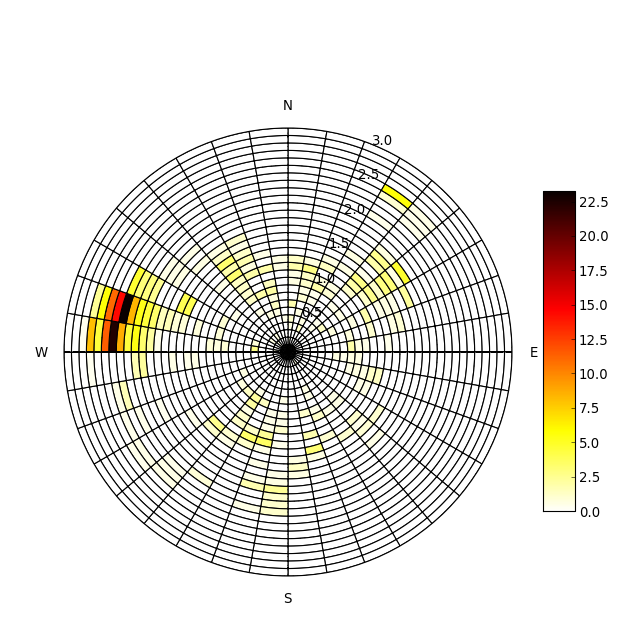
\includegraphics[width=.7\tw]{fig/05-Stapelung/beamforming_fk_analysis.png}
\caption{Beamforming Analyse von seismischen Wellen abgestrahlt von einer Hochhaussprengung in München. Aus ObsPy Gallerie (\url{http://docs.obspy.org/})}
\end{figure}

\subsection{Velocity Spectrum Analysis}
Die Richtung der ankommenden Wellenfront sei bekannt, aber der Betrag der Slowness  $|\vec{p}|$ und die Phasengeschwindigkeit $c_x$ seien unbekannt.
In diesem Fall kann die Geschwindigkeit-Spektrum-Analyse (eng. \textsl{Velocity Spectrum Analysis}) durchgeführt werden.\\
Dabei wird der Betrag der Slowness $|\hat{\vec{p}}|$, systematisch variiert, und jeweils wird ein Beam berechnet.
\[
Stack = f(\vert\hat{\vec{p}}\vert,t)
\]
Alle Hypothesen, jede Slowness, wird berechnet und erstellt daraus das Vespagramm.

\subsection{f-k-Analyse}
Die Frequenz-Wellenzahl Analyse kann auch berechnet werden um den Wellenzahlvektor zu berechnen.
Im Fall, das Geschwindigkeit und Richtung der Wellenfront unbekannt ist, kann eine Frequenz-Wellenzahl-Analyse durchgeführt werden. Dabei wird eine 3D-Fourier-Transformation durchgeführt:
\begin{equation}
u(k_{x},k_{y},\omega) = \iiint_{-\infty}^{\infty} u(x,y,t)\cdot e^{(-i(k_{x}x+k_{y}y+\omega t))} dxdyd\omega
\end{equation}
Das Modell (\textbf{für was?}) sei:
\[
u(x_{j},y_{j},\omega) = S(\omega)\cdot e^{(-ik\hat{r})}+N(x_{j},y_{j},\omega)
\]
{\small Dabei ist $S(\omega)\cdot e^{({-ik\hat{r}})}$ das empfangene Signal, $N(x_{j},y_{j},\omega)$ das Rauschen und $\vec{r}$ ist der Stationsvektor.}\\
Die Hypothese lautet:
\[
\hat{t_{j}} = \hat{\vec{p}} \vec{r}
\]
Stack im Frequenzbereich für alle mögliche $\vec{k}$.
Statt $u(k_{x}, k_{y}, \omega)$ nehmen wir $FK(\hat{\vec{k}},\omega)$ an, so erhalten wir:
\begin{equation}
FK(\hat{\vec{k}},\omega) = M_S(\omega)+\sum_j N(x_{j},y_{j},\omega)
\end{equation}
Anschließend können $k_{y}$- und $k_{x}$-Komponenten dargestellt werden und aus dem Plot der Wellenzahlvektor $\vec{k}$ abgelesen werden. So zeigt $\vec{k}$ die Richtung der einfallenden Wellenfront.
Weiter ist die Länge des Wellenzahlvektors in Relation zur slowness definiert als:
\begin{equation}
\vec{k} = \vec{n} k = \vec{n} \dfrac{\omega}{c_x} = \vec{n} \omega p= \omega \vec{p} 
\end{equation}
Aus der Richtung und der Länge des Wellenzahlvektors $\vec{k}$ berechnet man dann den Slownessvektor $\vec{p}$.\\
Eine wichtige Rolle bei der f-k-Analyse spielt das Auflösungsvermögen eines Arrays welche durch die Array-Antwort (eng. \textsl{Array Response}) beschrieben wird. Eine große Fläche des Arrays bedeutet eine hohe Auflösung im Wellenzahlbereich. Eine kleinere Fläche dagegen entspricht einer geringeren Auflösung. Bei einer geringen Stationsdichte entsteht bei f-k-Analyse kein klares Maximum im Wellenzahlbereich.\\
Modell: Im Ortsbereich nimmt man $u(x_j,y_j,t) = \delta(t-t_j)$ an, das entspricht $u(x_j,y_j,t)= e^{-i\omega t_{j}}$ im Frequenzbereich. Mit dem Stationsvektor $\vec{r_{j}}$ ist $u(x_j,y_j,t) = e^{-i\vec{k}\vec{r}_j}$  im Frequenzbereich.
Mit dem Verschiebungssatz folgt:
\begin{equation}
FK(\hat{\vec{k}},\omega) = \sum_{j} e^{i( \hat{k}-k)\vec{r_{j}}}
\end{equation}
Die 3D-Fourier Transformation liefert dann eine sinc-Funktion im Wellenzahlbereich. Ein Array, das im Ortsbereich  in $x$-Richtung gestreckt ist, zeigt eine elliptische Auflösung im Wellenzahlbereich.\\
Ein Array, das linear ausgerichtet ist, ist nicht optimal für die Frequenz-Wellenzahl-Analyse. Nur ein Array, das eine Fläche abdeckt zeigt ein eindeutiges Maximum im Wellenzahlbereich.

\chapter{Beamforming}

Bei Beamforming sucht man die richtige Wellenzahl $\vec{k}$ des Erdbebens, dabei wird die Stappelung von vielen Seismogrammen des gesuchten Bebens durchgeführt. 

Ein Seismogramm $u(x,y,t)$ kann als Funktion des zeitverschobenen Signals und Rauschen dargestellt werden:
\begin{equation}
u(x,y,t) = s(t-t_{j})+m(x_{j},y_{j},t)
\end{equation}
 Dabei ist $s(t-t_{j})$ das zeitverschobene Signal und $m(x_{j},y_{j},t)$ das Rauschen.\\
 Durch Summieren über alle Stationen wird ein Beam $b(t)$ erzeugt :
 
\begin{equation}
 b(t) = \sum_{j=1}^{n} u( x_{j},y_{j},t+t_{j})
\end{equation}
{\small Wobei $j$ der Stationindex ist.}\\\\ 
 Die Slowness sei bekannt. Für Slowness $\vec{p}$ gilt : $ \vec{p}\approx \hat{\vec{p}}$\\
 Die Zeitverschiebung ist: 
 \begin{equation}
 \hat{t}_{j}=\hat{\vec{p}}\hat{r}
 \end{equation}
Alle Seismogramme werden mit einer bestimmten Slowness verschoben. Der Prozess wird für alle Langsamkeiten , $\vec{p}$, durchgeführt. So wird die passende Wellenzahl der ankommenden Wellenfront wird ermittelt. 
 

 \begin{equation}
 b(t) = M_{s}(t)+ \sum_{j=1}^{n} u( x_{j},y_{j},t+t_{j})
 \end{equation}
 dabei ist $M_{s}(t)$ die konstruktive Interferenz und
\[
\sum_{j=1}^{n} u( x_{j},y_{j},t+t_{j})
\]
die destruktive Interferenz.

\section{Velocity Spectrum Analysis}
Die Richtung der ankommenden Wellenfront sei bekannt, aber der Betrag der Slowness  $\vert\vec{p}\vert$ und die Phasengeschwindigkeit $C_{x}$ seinen unbekannt.
In diesem Fall könnte die Geschwindigkeit-Spektrum-Analyse (\textit{Velocity Spectrum Analysis}) durchgeführt werden.\\
Dabei wird die Slowness, $|\hat{\vec{p}}|$, systematisch variiert, und jeweils wird ein Beam berechnet.
\[
Stack = f(\vert\hat{\vec{p}}\vert,t)
\]
Alle Hypothese, jede Slowness, wird berechnet und erstellt daraus das Vespagramm. 

\section{f-k-Analyse}
Die Frequenz-Wellenzahl Analyse kann auch berechnet werden um den Wellenzahlvektor zu berechnen.
Im Fall, das Geschwindigkeit und Richtung der Wellenfront unbekannt ist, kann eine Frequenz-Wellenzahl-Analyse durchgeführt werden. Dabei wird eine 3D-Fourier-Transformation durchgeführt:
\begin{equation}
u(k_{x},k_{y},\omega) = \iiint_{-\infty}^{\infty} u(x,y,t)\cdot\exp^{(-i(k_{x}x+k_{y}y+\omega t))} dxdyd\omega
\end{equation}
Das Modell (\textbf{für was?}) sei:
\[
u(x_{j},y_{j},\omega) = S(\omega)\cdot\exp^{(-ik\hat{r})}+N(x_{j},y_{j},\omega)
\]
{\small Dabei ist $S(\omega)\cdot\exp({-ik\hat{r}})$ das empfangene Signal, $N(x_{j},y_{j},\omega)$ das Rauschen und $\vec{r}$ ist der Stationsvektor.}\\
Die Hypothese lautet:
\[
\hat{t_{j}} = \hat{\vec{p}} \vec{r}
\]
Stack im Frequenzbereich für alle mögliche $\vec{k}$.
Statt $u(k_{x}, k_{y}, \omega)$ nehmen wir $FK(\hat{\vec{k}},\omega)$ an, so erhalten wir:
\begin{equation}
FK(\hat{\vec{k}},\omega) = M S(\omega)+\sum_{j}N(x_{j},y_{j},\omega)
\end{equation}
Anschließend können $k_{y}$- und $k_{x}$-Komponenten dargestellt werden und aus dem Plot der Wellenzahlvektor $\vec{k}$ abgelesen werden. So zeigt $\vec{k}$ die Richtung der einfallenden Wellenfront.
Weiter ist die Länge des Wellenzahlvektors in relation zur slowness definiert als:
\begin{equation}
\vec{k} = \vec{n} k = \vec{n} \dfrac{\omega}{c_x} = \vec{n} \omega p= \omega \vec{p} 
\end{equation}
Aus der Richtung und der Länge des Wellenzahlvektors $\vec{k}$ berechnet man dann den Slownessvektor $\vec{p}$.\\
Eine wichtige Rolle bei der f-k-Analyse spielt das Auflösungsvermögen eines Arrays. Die Array-Antwort beschreibt die Auflösungsvermögen einers Arrays. Grosse Fläche des Arrays bedeutet eine hohe Auflösung im Wellenzahlbereich. Dagegen eine kleinere Fläche entspricht einer geringeren Auflösung. Bei einer geringen Stationsdichte entsteht bei f-k-Analyse kein klares Maximum im Wellenzahlbereich.
Modell: Im Ortsbereich nimmt man $u(x_{j},y_{j},t) = \delta(t-t_{j})$ an, das ist $u(x_{j},y_{j},t)= \exp^{-i\omega t_{j}}$ im Frequenzbereich. Mit dem Stationsvektor $\vec{r_{j}}$ ist $u(x_{j},y_{j},t) = \exp^{-i\vec{k}\vec{r_{j}}}$  im Frequenzbereich.
Mit dem Verschiebungssatz folgt:
\begin{equation}
FK(\hat{\vec{k}},\omega) = \sum_{j}\exp^{i( \hat{k}-k)\vec{r_{j}}}
\end{equation}
3D-Fourier-Transformation liefert dann eine sinc-Funktion im Wellenzahlbereich. Ein Array, das im Ortsbereich  in $x$-Richtung gestreckt ist, zeigt eine elliptische Auflösung im Wellenzahlbereich.\\
Ein Array, das linear ausgerichtet ist, ist nicht optimal für die Frequenz-Wellenzahl-Analyse. Nur ein Array, das eine Fläche abdeckt zeigt ein eindeutiges Maximum im Wellenzahlbereich.

\chapter{Korrelation}

\section{Kreuzkorrelationsfunktion}

In der Signalanalyse beschreibt die Kreuzkorrelationsfunktion (KKF) die Korrelation zweier Signale $x(t)$ und $y(t)$ bezüglich einer Zeitverschiebung.\\

Deterministisch \textit{kontinuierlich}
\begin{equation}
\delta{xy}(t) = \int_{-\infty}^{\infty} x(t') y(t'+t) dt
\end{equation}
{\small Mitunter hat die Korrelation ein anderes Vorzeichen, d.h. $t'+t \equiv t'+t$}\\\\

Deterministisch \textit{diskret}
\begin{equation}
R_{xy}(j) = \sum_i x_i y_{i+j}
\end{equation}

Die Normierte Kreuzkorrelationsfunktion
\begin{equation}
R_{xy}(t) = \frac{1}{T_x} \int_{-\infty}^{\infty} x(t') y(t'+t) dt
\end{equation}
{\small Wobei $T_x$ die Länge des Signals $x(t)$ ist.}


\section{Autokorrelationsfunktion}
Die Autokorrelationsfunktion (AKF) bestimmt die Korrelation eines Signals mit sich selbst. Die Korrelation wird analog zur Kreuzkorrelation gebildet.

\subsection{AKF eines stochastischen Prozesses}
Betrachten wir die Autokorrelations als einen stochastischen Prozess in dem der Erwartungswert, $E$, des Signals $x(t)$ angenommen werden kann als
\begin{align*}
E[x^2(t)] & < \infty,\\
E[x(t)] & = 0.
\end{align*}
Dann sind die Erwartungswerte der Autokorrelation des Signals $x(t)$
\[
R_{xx}(t) = E[x(t_1)\,x(t_2)].
\]
Liegt eine schwache Stationalität des gemessenen Signals vor ist die Autokorrelation
\[
R_{xx}(t_1, t_2) = R_{xx}(t+t_1, t+t_2)
\]
{\small $\forall\,t, t_1, t_2$}\\\\
Die \textit{Autokovarianzfunktion} ist so nur vom Timelag $\tau = t_2 - t_1$ abhängig,
\[
R_{xx}(t_1, t_1+\tau) = R_{xx}(\tau) = E[x(t), x(t+\tau)].
\]
Das führt zur zu folgendem Ausdruck der Autokorrelationsfunktion:
\begin{equation}
R_{xx}(\tau) = \frac{R_{xx}(\tau)}{R_{xx}(0)}
\end{equation}


\subsection{Schätzung der AKF}
Die Schätzung der Autokorrelationsfunktion mithilfe von diskreten Realisierungen kann geschrieben werden als Normierte Summe
\[
\hat R_{xx}(i) = \frac{1}{N-i} \sum_{j=0}^{N-i} x_j\,x_{j+i}
\]
Die \textit{erwartungstreue} Schätzung der Korrelation
\[
E[\hat R_{xx}(i)] = \frac{1}{N-i} \sum_{j=0}^{N-i} E[x_j,\,x_{j+i}]
\]

\section{Korrelation und Faltung}
Vergleicht man die Faltung mit Korrelationsfunktion zeigen sich folgende Identitäten
\[
F\{x(t) \ast y(t)\} = x(\omega)\,y(\omega) = |X(\omega)| |Y(\omega)|\,e^{\varphi_x(\omega) + \varphi_y(\omega)},
\]
dies führt zu
\[
F\{R_{xy}\} = x(\omega)\,y^*(\omega) = |X(\omega)| |Y(\omega)|\,e^{\varphi_x(\omega) - \varphi_y(\omega)}.
\]
Man beachte den Vorzeichenwechsel des Phasenantherms.

\subsection*{Faltung der geraden AKF}
Die Faltung der geraden Autokorrelationsfuntion. Wir nehemen an, dass
\[
R_{xx}(t) = R_{xx}(-t).
\]
Dies führt zu zu folgender Identität
\[
F\{R_{xx}(t)\} = |X(\omega)|^2 \Rightarrow \textrm{Powerspektrum}.
\]

\section{Beispiele für Korrelationen}

\subsection*{AKF eines Boxcars}
Die Autokorrelation einer Boxcarfunktion.
\begin{figure}[h!]
\centering
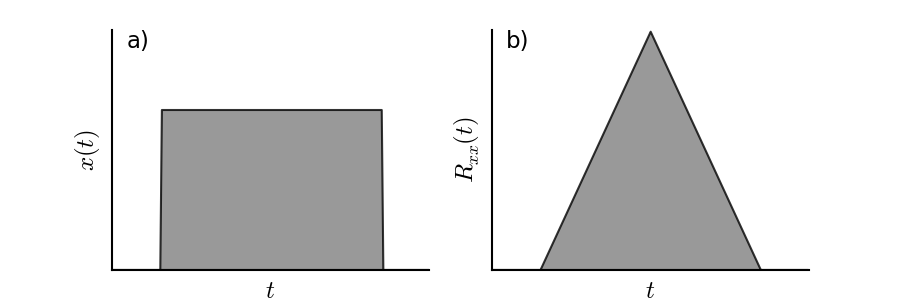
\includegraphics[width=.9\tw]{fig/09-Korrelation/01-example_boxcar.png}
\caption{Schematisches Beispiel der Boxcarfunktion (a) und Autokorrelation derselbigen Boxcarfunktion (b).}
\end{figure}
\begin{align*}
R_{xx}(t) & = \int_{-\infty}^\infty x(t') x(t'+t) dt' \\
& = \begin{cases}
 \int_t^T dt' & -T \leq t \leq 0\\
 \int_0^{T-t} dt' & 0  \leq t \leq T\
 \end{cases}
\end{align*}


\subsection*{AKF einer Deltafunktion}
Die Autokorrelationsfunktion einer Deltafunktion, $x(t) = \delta(t)$
\begin{align*}
R_{xx}(t) & = \int_{-\infty}^\infty \delta(t') \delta(t'+t) dt'\\
& = \sigma(t)
\end{align*}

\subsection*{Überlagerte Deltafunktionen}
Überlagerung zweier Deltafunktionen mit Amplitude $\delta(t_1) = a$ und $\delta(t_0) = b$ führt zu
\[
R_{xx}(t) = (a^2 + b^2)\delta(t) + ab(\delta(t-t_0) + \delta(t+t_0)).
\]

\begin{figure}[h!]
\centering
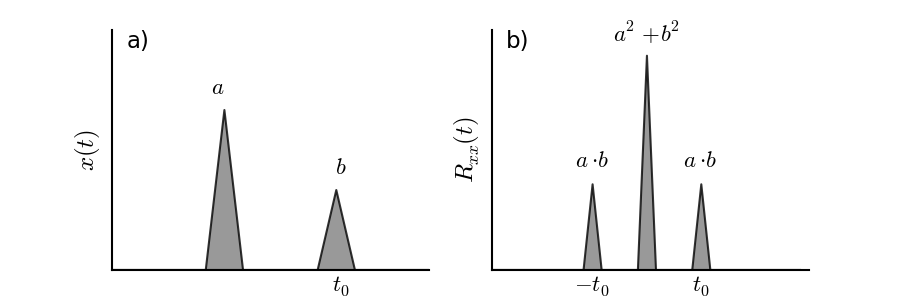
\includegraphics[width=.9\tw]{fig/09-Korrelation/02-example_deltafct.png}
\caption{Schematisches Beispiel zweier Deltafunktionen (a) und Autokorrelation derselbigen Deltafunktpeaks (b).}
\end{figure}

\subsection*{AKF bei Nullzahliger Verschiebung}
Die AKF einer Funktion bei $t=0$ folgt:
\[
R_{xx}(0) = \int_{-\infty}^\infty \delta(t')\,\delta(t') dt' = \int_{-\infty}^\infty \delta(t')^2 dt'.
\]


\section*{AKF einer harmonischen Schwingung}
Betrachten wir die Schwingung
\[
x(t) = \sin(\omega_0 t)
\]
und die Autokorrelation dieser harmonischen Funktion:
\[
R_xx(t) = \frac{1}{T} \int_{-\infty}^\infty x(t') x(t'+t) dt'
\]
\begin{figure}[h!]
\centering
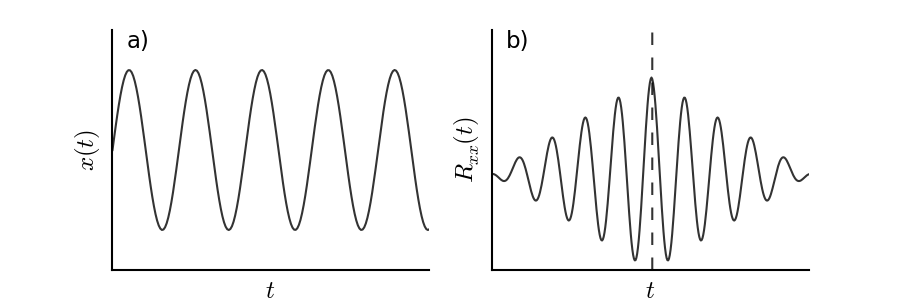
\includegraphics[width=.9\tw]{fig/09-Korrelation/03-example_harmonic.png}
\caption{Schematisches Beispiel einer harmonischen Schwingung (a) und Autokorrelation (b).}
\end{figure}

\section*{AKF Gaußsche Glockenkurve}
Autokorrelation einer Gaußschen Glockenkurve der Form
\[
x(t) = a\,e^{-t^2/2T^2},
\]
führt zu
\[
R_{xx}(t) = a^2 T \sqrt{\pi} e^{-t^2/4T^2}.
\]

\section*{AKF eines Sweeps}
Autokorrelation eines Sweeps der Form
\[
\mbox{sweep}(t)=
\begin{cases}
\sin \left(2\pi \left(v_1 + \frac{v_1-v_2}{T} t \right)\right) & t \leq T\\
0& sonst
\end{cases}
\]

Abbildung \ref{fig:korr_sweep} zeigt einen schematischen Sweep und dessen Autokorrelation

\begin{figure}[h!]
\centering
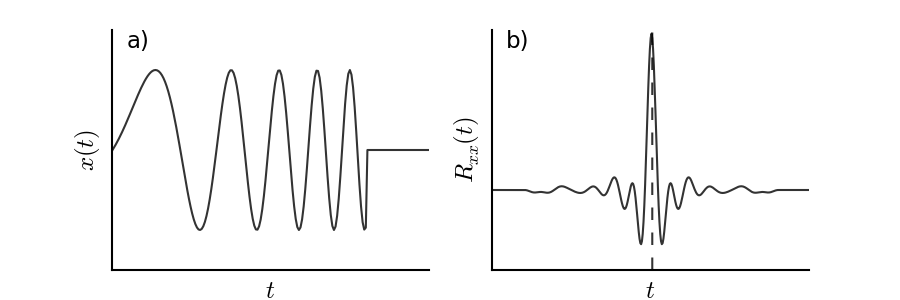
\includegraphics[width=.9\tw]{fig/09-Korrelation/04-example_sweep.png}
\caption{Schematisches Beispiel einer Sweep Funktion (a) und dessen Autokorrelation (b).}
\label{fig:korr_sweep}
\end{figure}

\section*{AKF von Weißem Rauschen}
Die Autokorrelation von weißem Rauschen,
\[
\{u_i\} = \mbox{iid}.
\]
{\small iid: Independent and identically distributed}\\\\
So folgt die AKF für weißes Rauschen:
\[
R_{uu}(i) = E[u_j + u_{j+i} =
\begin{cases}
\sigma u^2 & i=0\\
0 & \mbox{sonst}
\end{cases}
\]
{\small $\sigma$ ist die Varianz der Amplitude des weißen Rauschens}

\section*{AKF von farbigem Rauschen}
Farbiges Rauschen ist gleichverteiltes Rauschen in einem begrenzten Frequenzband.
\[
F\{R_{xx}(i)\} = \mbox{const.} = |N(\omega)|^2
\]

\section*{AKF einer Seismischen Spur}
Formeln müssen überarbeitet werden!\\\\

Die Autokorrelation einer Seismischen Spur $s$ kann betrachtet werden als
\[
s_i = w_i * x_i.
\]
{\small Dabei ist $w_i$ das Wavelet und $x_i$ die Reflektivität.}
$x_i$ ist gleichverteilt:
\begin{align*}
\{x_i\} = \mbox{iid ZP} & & R_{xx}(i) = \sigma x^2 \, \sigma(\hat{t})^2
\end{align*}
{\small iid ZP: unabhängiger Zufallsprozess}\\
Dann ist der Erwartungswert der Autokorrelation des Signals:
\begin{align*}
R_{ss}(i) & = E[s_j\, s_{j+i}]\\
& = E\left[\sum_k w_k, x_{j-k}\, \sum_l w_l x_{j+i-l}\right]\\
& = \sum_k \sum_l w_l\,E[x_{j-k}\,x_{j+i-l}]\\
& \not= 0
\begin{cases}
Nur & j-k = j+i-l\\
Oder & l = i+k
\end{cases}
\end{align*}

Daraus folt, dass die Autokorrelation der Seismischen Spur etwa der Autokorrelation des Wavelets entspricht:
\[
R_{ss}(i) \sim R_{ww}(i) = \sigma x^2 \, \sum_k w_k \, w_{k+1} < \sigma x^2 R_{ww}(i)
\]
So kann der Frequenzgehalt des initialen Wavelets aus der Seismischen Spur oder Seismogramm abgelesen werden.

\section*{AKF Seismische Spur mit Ghost}
Autokorrelation einer Seismischen Spur mit Ghost.
\[
y_i = s_i * g_i.
\]
{\small Wobei $g_i$ der Ghostoperator ist}\\
Im Frequenzbereich:
\[
Y(\omega) = S(\omega) \cdot G(\omega)
\]
So ist die Fouriertransformierte der Autokorrelation
\begin{align*}
F\{R_{yy}(i)\}\;Y(\omega)\,Y*(\omega) & = S(\omega) G(\omega) S*(\omega) G*(\omega)\\
& = F\{R_{gg}\},
\end{align*}
was uns zu
\[
R_{yy}(i) = R_{ss}(i)*R_{gg}(i)
\]
führt.

\end{document}
